\documentclass[times, utf8, diplomski]{fer}
\usepackage{booktabs}
\usepackage{mathtools}
\usepackage{amsmath}
\usepackage{amsthm}
\usepackage{stackengine}
\usepackage[]{algorithm2e}
\usepackage{booktabs}
\usepackage{float}
\newtheorem{prop}{Propozicija}
\newtheorem{theorem}{Teorem}
\graphicspath{ {Slike/} }
\begin{document}

% TODO: Navedite broj rada.
\thesisnumber{1544}

\title{Polunadzirana klasifikacija rukom pisanih znakova generativnim suparničkim modelima}

\author{Marko Jelavić}

\maketitle

% Ispis stranice s napomenom o umetanju izvornika rada. Uklonite naredbu \izvornik ako želite izbaciti tu stranicu.
\izvornik

\zahvala{Zahvaljujem se mentoru, izv. prof. dr. sc. Siniši Šegviću na podršci i vodstvu kroz diplomski studij te na savjetima i pomoći prilikom izrade diplomskog rada.}

\tableofcontents

\chapter{Uvod}
Klasifikacija rukom pisanih znakova se često koristi kao uvodni problem u područje računalnog vida. Najpoznatiji takav problem je klasifikacija rukom pisanih znamenki (\cite{mnist}) gdje se svakoj slici mora pridijeliti pripadajuća znamenka kao klasa. Pošto se radi o maloj bazi podataka slika niskih rezolucija, rezultati se mogu brzo dobiti te se novi modeli najčešće provjeravaju nad njom. Modeli koji uspješno obavljaju klasifikaciju rukom pisanih znakova najčešće primjenu nalaze kao dio sustava za pretraživanje informacija iz dokumenata. \par

Duboki diskriminativni modeli se smatraju najsuvremenijom tehnologijom iz razloga što pružaju najbolje rezultate u širokom spektru primjena te su najzaslužniji za ekspanziju primjene umjetne inteligencije u industriji. Mana takvih modela je ta što zahtijevaju ogroman broj ručno označenih podataka da bi postigli zadovoljavajuće rezultate. Označavanje podataka je izrazito skup proces te ga se nastoji zaobići. \par

S druge strane, duboki generativni modeli ne zahtijevaju veliku količinu označenih podataka. No, problemi s dosadašnjim modelima se javljaju pri aproksimacijama vjerojatnosnih izračuna pri modeliranju vjerojatnosti ulaznih podataka što usporava proces treniranja modela (\cite{GAN}). U navedenom radu predlaže se model koji se zasniva na suparničkim neuronskim mrežama. 

Model generativnih suparničkih mreža se sastoji od dviju neuronskih mreža, generatorske i diskriminatorske. Spada pod familiju modela bez učitelja, odnosno nisu mu potrebni označeni primjeri za učenje, već samo uči distribuciju ulaznih podataka. Mreža generator ima zadatak naučiti distribuciju ulaznih podataka, a to čini provođenjem latentnih varijabli na ulazu kroz svoje slojeve te kao izlaz daje sliku poput primjera za učenje. Mreža diskriminator ima zadatak odrediti da li je primjer na njenom ulazu generiran ili stvaran. Kroz postupke optimizacije težina, istovremeno se poboljšavaju generator i diskriminator. \par

Nije dugo trebalo da se ovaj model, kao i većina generativnih, pokuša preformulirati u polunadzirani model, te da u konačnici služi kao klasifikator. Pokazalo se da za manji broj ulaznih podataka model funkcionira bolje od izoliranog klasifikatora (\cite{odena}). Upravo to je i cilj ovog rada koji ima zadatak dati uvid u najpoznatije inačice generativnih suparničkih modela, te isprobati model u polunadziranom okruženju na novoj bazi primjera za učenje. \par

Poglavlje 2 daje uvod u neuronske mreže te obrazloženje odabranih pojmova u tom polju, generativne suparničke mreže s teoretske strane su obrađene u poglavlju 3, dok poglavlje 4 prezentira rezultate eksperimenata sa slikama i mjerenjima uz popratne komentare. Zaključak rada se nalazi u poglavlju 5, a literatura je prikazana na samom kraju prije sažetka. \par

\chapter{Neuronske mreže}
Umjetne neuronske mreže nastale su kao simulacija rada ljudskog mozga. Skupina umjetnih neurona koji su međusobno povezani zajedno čine neuronsku mrežu. Svaki od neurona procesira informaciju na ulazu te daje izlaz. Grupiranje više neurona omogućava modeliranje složenijih relacija koji postoje u podacima na ulazu. Arhitektura neuronske mreže određuje način na koji su umjetni neuroni u istoj spojeni. Također, svaki od neurona može na više načina procesirati ulaze. Neuronske mreže stoga predstavljaju izrazito konfigurabilan model strojnog učenja, koji nalazi široku primjenu u polju umjetne inteligencije.

\section{Umjetni neuron}
Osnovni model umjetnog neurona postavljen je 1940-ih \cite{mcculloch}. Sastoji se od ulaza u neuron koji su težinski povezani s istim, zatim se otežani ulazi zbrajaju, te se primjenjuje aktivacijska funkcija neurona, kao što je prikazano na slici 2.1. \par

\begin{figure}[!htbp]
    \centering
    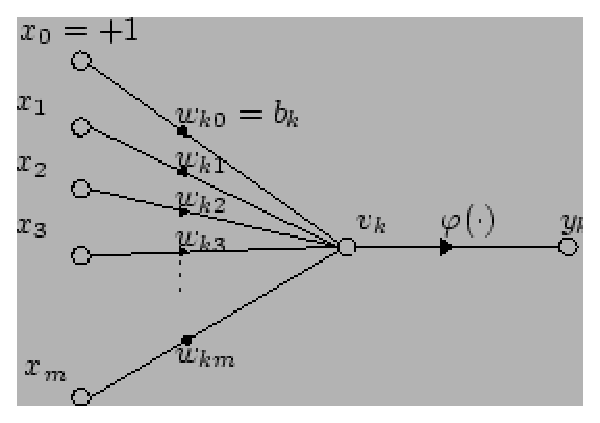
\includegraphics[scale=0.8]{Slike/Artificial_neuron}
    \caption{Umjetni neuron \cite{neuron}}
\end{figure}

Pošto je svim neuronima zajedničko otežano zbrajanje ulaza, svojstva pojedinog neurona zapravo najviše ovise o njegovoj aktivacijskoj funkciji. O njima više u idućoj sekciji.

\subsection{Aktivacijske funkcije}
Aktivacijske funkcije su najznačajnija karakteristika svakog neurona, stoga ne čudi da napredak u razumijevanju pojedinih aktivacijskih funkcija, te predlaganje novih često dovodi do napretka u neuronskim mrežama.

\subsubsection{Prag}
Funkcija praga predložena je u algoritmu Perceptrona \cite{perceptron}. Koristi se kao binarni klasifikator. Model Perceptrona je linearan, što znači da algoritam nije u mogućnosti ispravno klasificirati ni najjednostavnije linearno neseparabilne probleme poput prikazanog na slici 2.2. Ta tvrdnja je i dokazana \cite{minsky}.

\begin{figure}[!htbp]
    \centering
    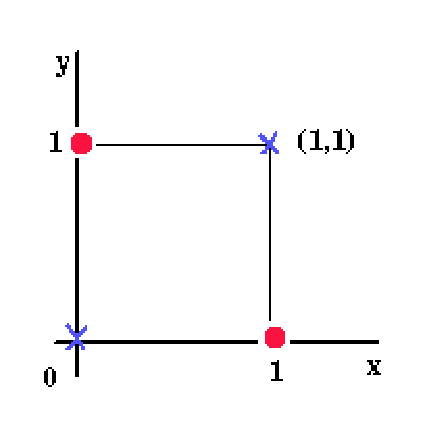
\includegraphics{Slike/xorGraph}
    \caption{XOR problem \cite{xor}}
\end{figure}

Nakon sumiranja otežanih ulaza, funkcija praga se primjenjuje po izrazu 2.1, a graf funkcije je vidljiv na slici 2.3.

\begin{equation}
    f(x)=
    \begin{cases}
      1, & x \geq 0 \\
      0, & x < 0
    \end{cases}
\end{equation}

\pagebreak

\begin{figure}[htbp]
    \centering
    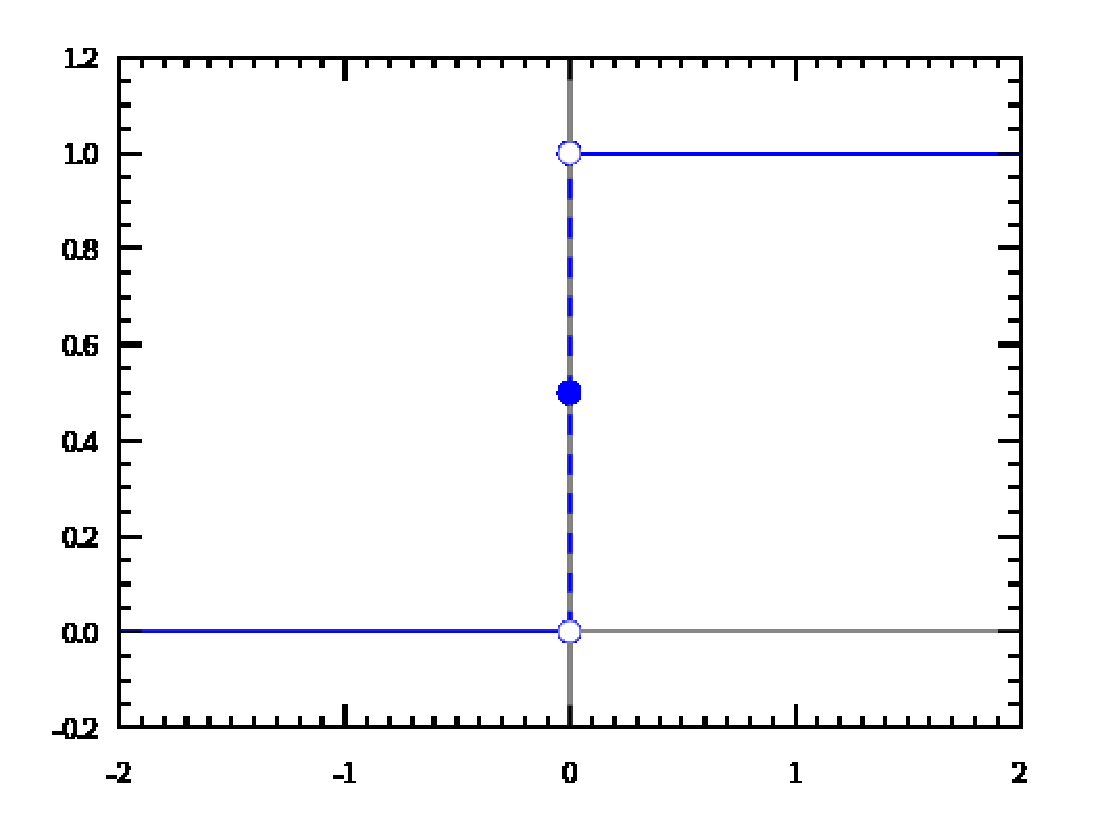
\includegraphics[scale=0.5]{Slike/step}
    \caption{Funkcija praga \cite{step}}
\end{figure}

\subsubsection{Sigmoidalna funkcija}
Sigmoidalna funkcija se prvotno koristila u logističkoj regresiji, te sama logistička regresija može bit interpretirana kao neuron kojem je aktivacijska funkcija sigmoidalna funkcija. Logistička regresija je također linearan klasifikator, no svoju značajnost za razliku od funkcije praga poprima u neuronskim mrežama. \par

Sigmoidalna funkcija je nelinearna aktivacijska funkcija. U neuronskim mrežama izlaz jednog neurona je ulaz drugome. Uvođenjem nelinearnosti preko aktivacijske funkcije omogućava se modeliranje kompleksnijih relacija od linearnih, te širenje primjene modela i na linearno neseparabilne probleme. Zadana je jednadžbom 2.2, a slika 2.4 prikazuje graf funkcije te graf njene derivacije. \par

\begin{equation}
    f(x)=\frac{1}{1 + e^{-x}}
\end{equation}

\begin{figure}[htbp]
    \centering
    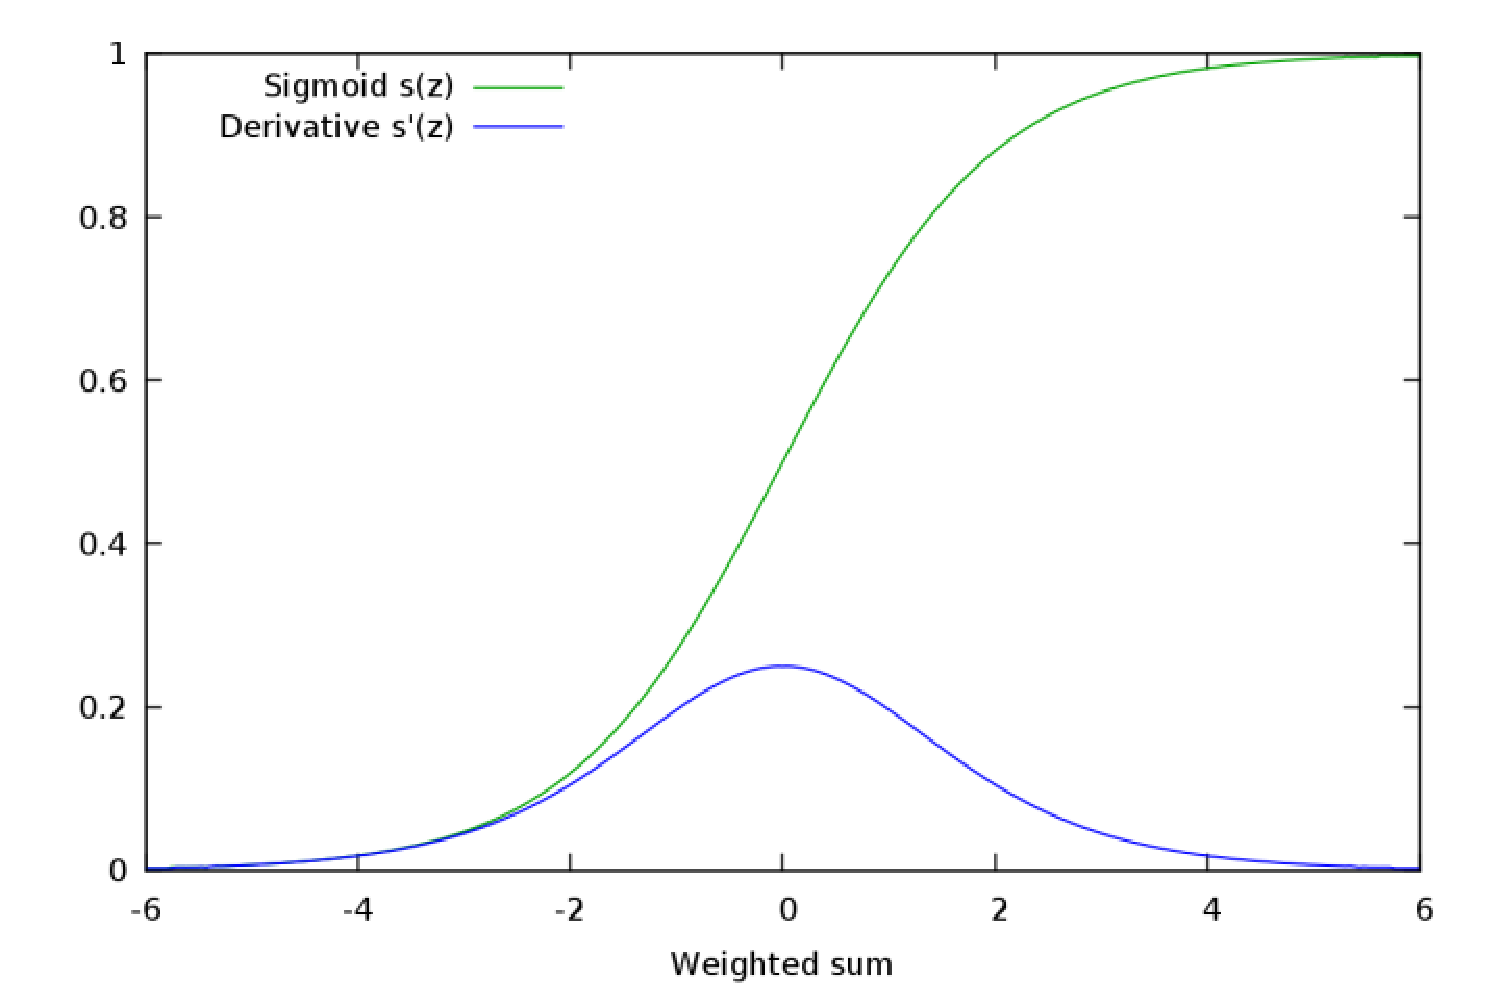
\includegraphics[scale=0.3]{Slike/sigmoid}
    \caption{Sigmoidalna funkcija \cite{sigmoid}}
\end{figure}

Iz grafa funkcije je vidljivo da se sigmoidalnom funkcijom dobije pouzdanost klasifikacije neurona za određeni primjer, što je korisna informacija. No, prva derivacija otkriva manu, a to je problem nestajućeg gradijenta. Ukoliko je izlaz neurona primjerice 0.99, odnosno klasa 1, a zapravo bi trebao biti klasa 0, gradijent je izrazito mali, što znači da će za korekciju klasifikacije trebati velik broj iteracija algoritma gradijentnog spusta.

\subsubsection{Tangens hiperbolni}
Tangens hiperbolni kao aktivacijska funkcija se počeo češće koristiti kao zamjena za sigmoidalnu funkciju iz razloga što ona daje isključivo pozitivne izlaze u intervalu $[0, 1]$ te je centrirana oko $0.5$. To ne predstavlja problem samo jednom neuronu, dok u višeslojnoj neuronskoj mreži koči brzinu konvergencije u postupku učenja. Stoga se predlažu funkcije centrirane oko $0$, a upravo jedna od takvih je tangens hiperbolni \cite{efficient}. Funkcija je zadana jednadžbom 2.3, a graf funkcije i njene derivacije je vidljiv na slici 2.5.

\begin{equation}
    f(x)=tanh(x)=\frac{sinh(x)}{cosh(x)}=\frac{1 - e^{-2x}}{1 + e^{-2x}}
\end{equation}

\begin{figure}[htbp]
    \centering
    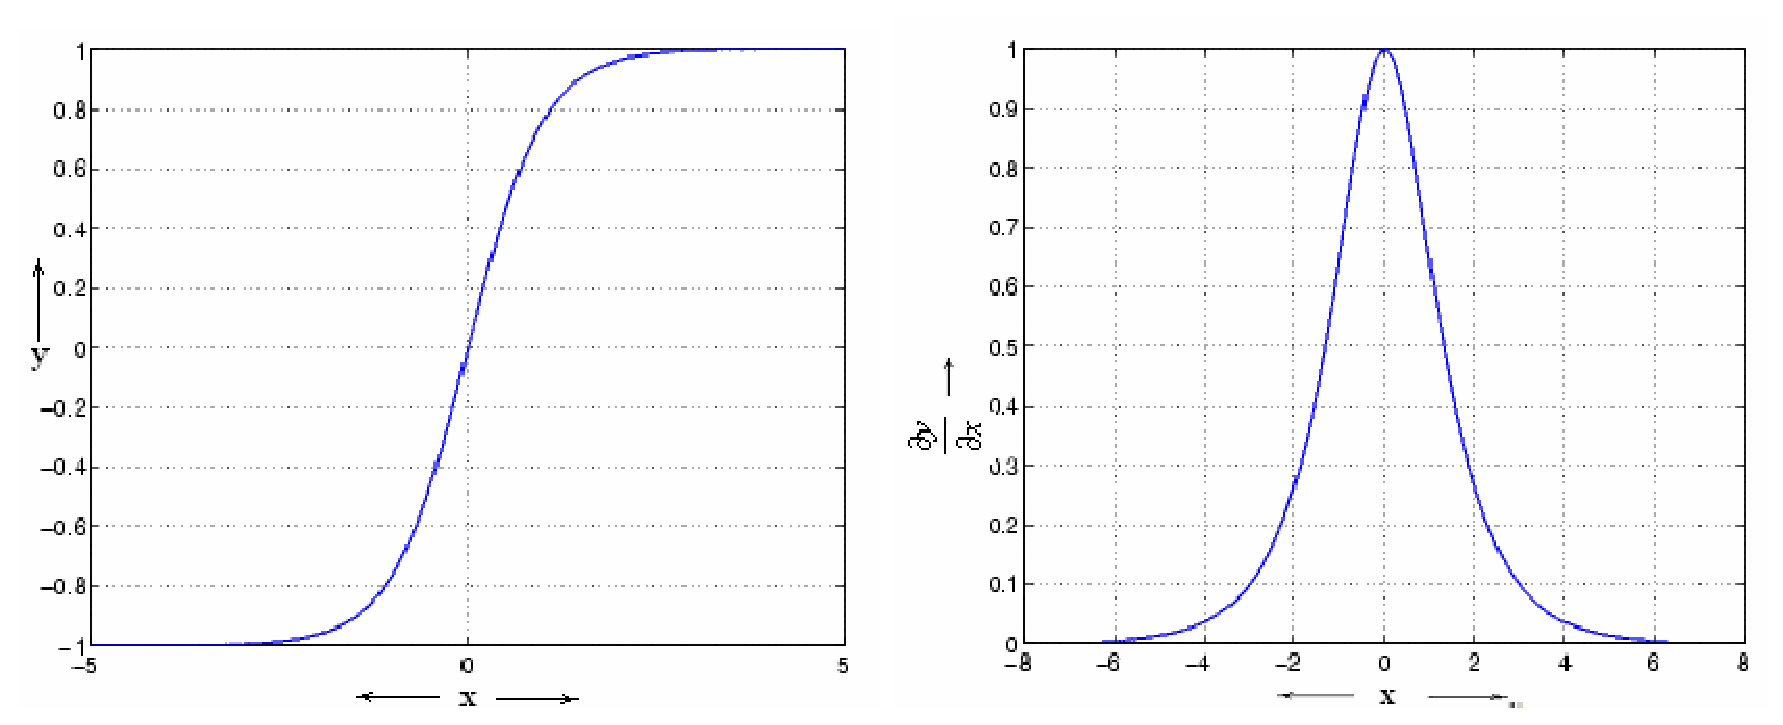
\includegraphics[scale=0.5]{Slike/tanh}
    \caption{Tangens hiperbolni \cite{tanh}}
\end{figure}

Predložena je i modifikacija aktivacijske funkcije u izraz \cite{efficient}:

\begin{equation}
    f(x)=1.7159 tanh\left( \tfrac{2}{3}x \right).
\end{equation}

Modificirana funkcija za ulaze koji su centrirani na $0$, sa varijancom $1$, daje izlaze koji su također centrirani na $0$ i varijanca bi im trebala biti blizu $1$.

\subsubsection{Zglobnica}

U kontekstu neuronskih mreža, zglobnica je aktivacijska funkcija čija formula glasi:

\begin{equation}
    f(x)=max(0,x)
\end{equation}

Trenutno je najpopularnija aktivacijska funkcija u arhitekturama dubokih neuronskih mreža (\cite{rect}). Izračunski je vrlo jednostavna, te njen gradijent također ( $0$ za $x<0$, $1$ za $x>0$, nediferencijabilan u $0$), dovodi i do rjeđih aktivacija neurona. Potencijalni problemi su: nije centrirana oko $0$, nediferencijabilna u $0$, neograničena aktivacija te se zna dogodit fenomen umirućih neurona, odnosno neuroni se dovedu u mrtvo stanje iz kojeg ne mogu više izaći, efektivno smanjujući kapacitet neuronske mreže \cite{rect}. Diferencijabilnost u $0$ se rješava tako što se definira da gradijent u $0$ bude ili $0$ ili $1$, neograničenu aktivaciju pod kontrolom drži grupna normalizacija koja najčešće prethodi aktivacijskoj funkciji, a fenomen umirućih neurona rješavamo parametriziranom zglobnicom (2.6) gdje se za odabir $a$ često uzima vrijednost u intervalu $<0, 1>$. Slika 2.6 prikazuje zglobnicu.

\begin{figure}[htbp]
    \centering
    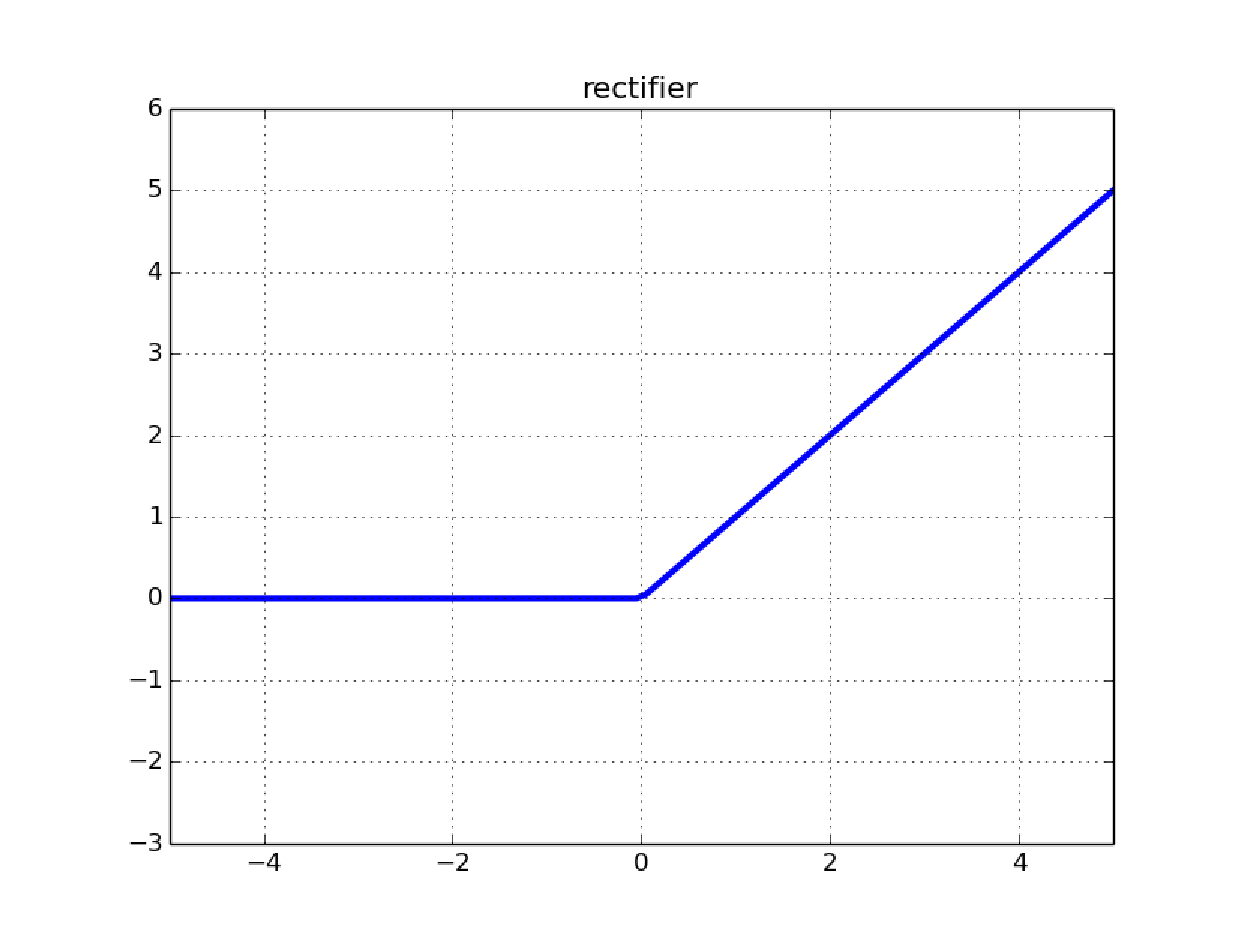
\includegraphics[scale=0.5]{Slike/rect}
    \caption{Zglobnica \cite{rectpic}}
\end{figure}

ReLU je lesto korištena skraćenica za zglobnicu. Poznate varijante su Parametric ReLU (2.6) i ELU (2.7) \cite{rect}.

\begin{equation}
    f(x)=
    \begin{cases}
      x, & x > 0 \\
      ax, & otherwise
    \end{cases}
\end{equation}

\begin{equation}
    f(x)=
    \begin{cases}
      x, & x \geq 0 \\
      a(e^x - 1), & otherwise
    \end{cases}
\end{equation}

\section{Višeslojni perceptron}
Općenita unaprijedna neuronska mreža najčešće se naziva i višeslojnim perceptronom. Sadrži 3 vrste slojeva: ulazni, skriveni i izlazni. Ima 1 ulazni i 1 izlazni sloj, a skrivenih može biti po volji mnogo. Ilustracija jednog višeslojnog perceptrona dana je na slici 2.7.

\begin{figure}[htbp]
    \centering
    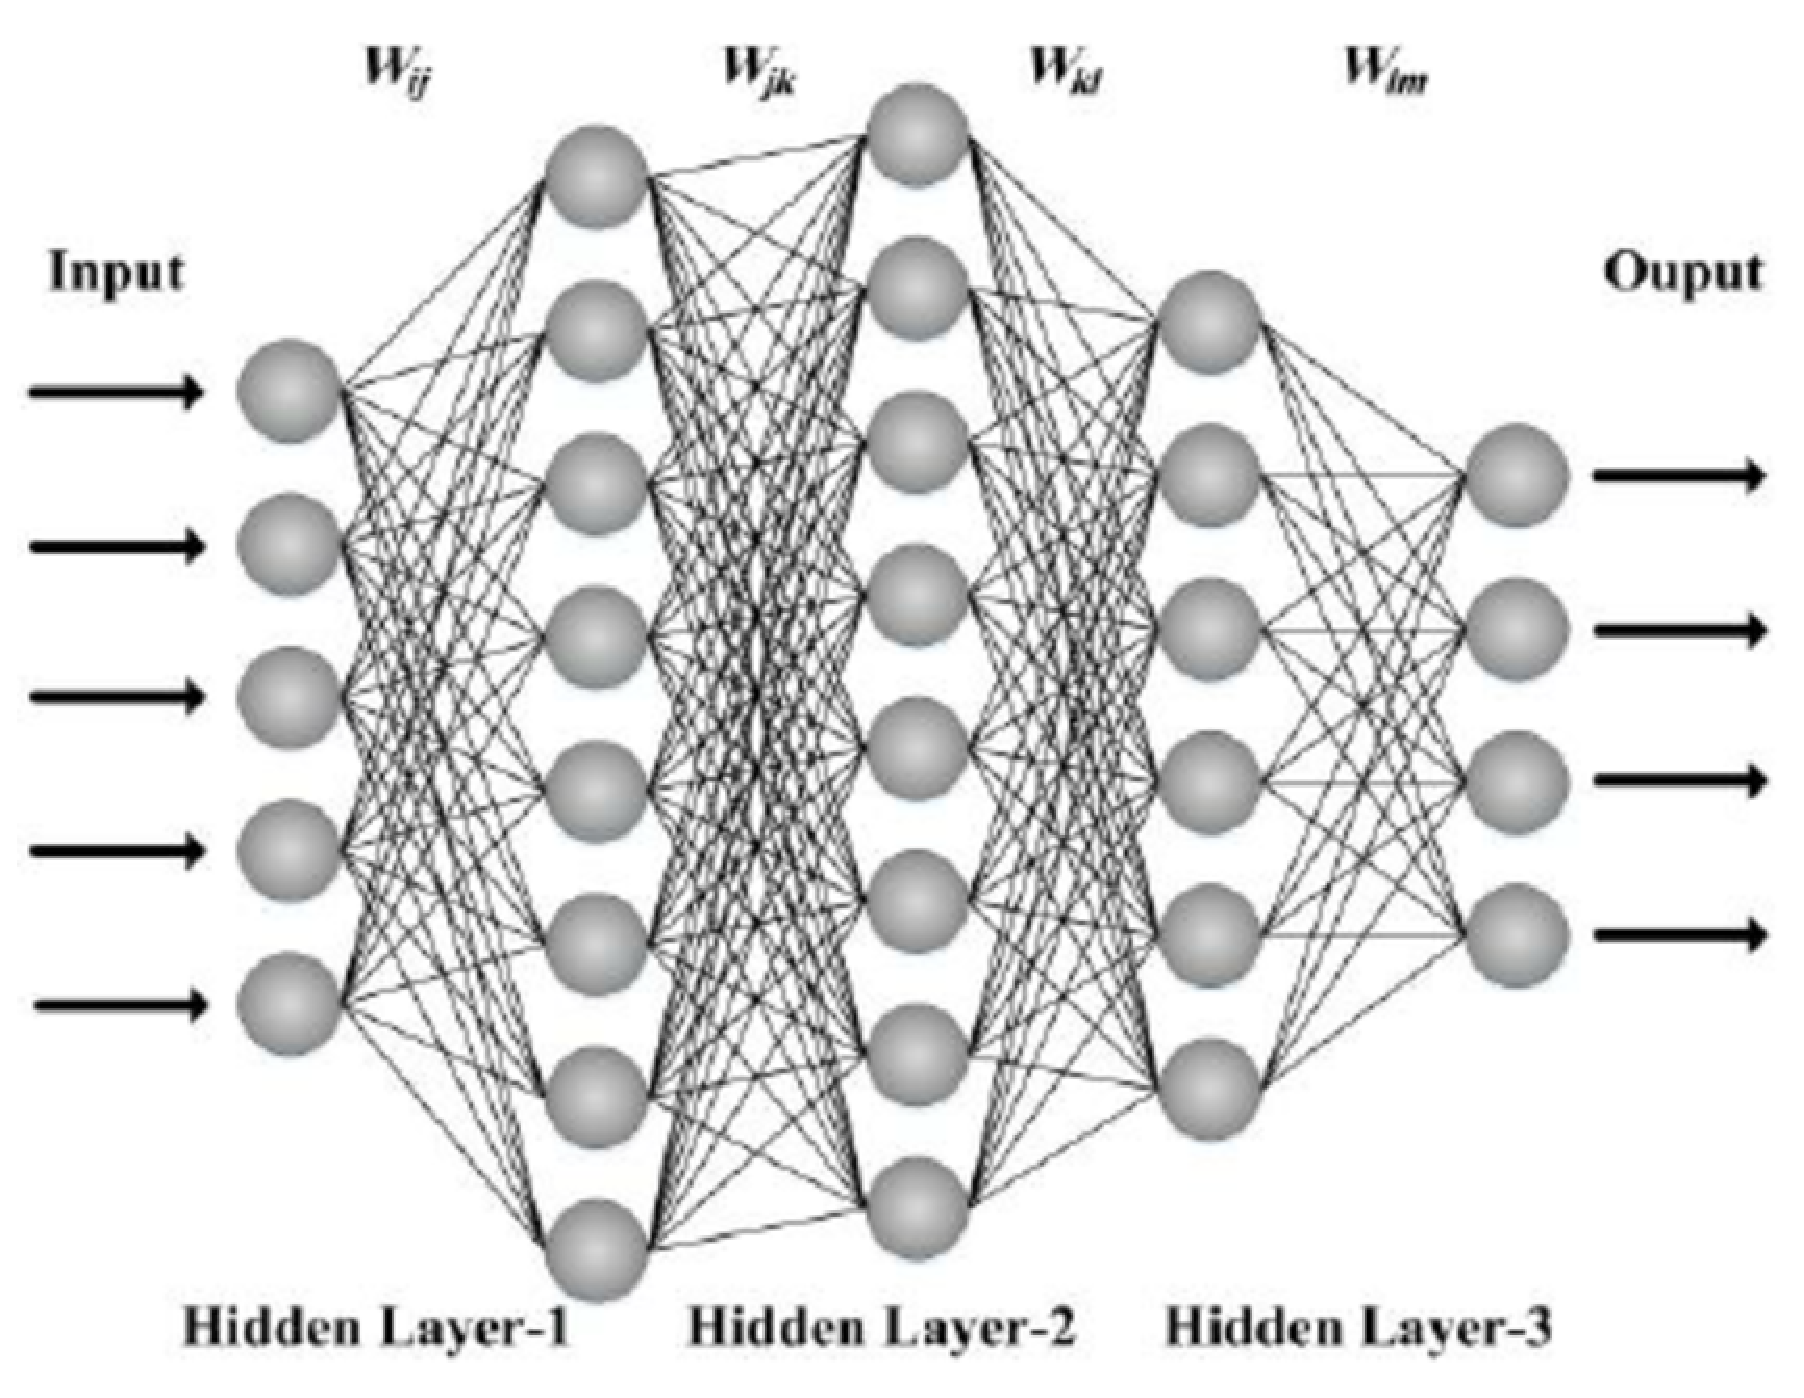
\includegraphics[scale=0.4]{Slike/mlp}
    \caption{Višeslojni perceptron \cite{mlp}}
\end{figure}

Ulazni sloj predstavlja značajke podataka koje obrađujemo, na primjer za sliku, svaki pojedini neuron bi bio jedan piksel slike. U njima se ne vrši nikakva obrada već se samo proslijede prvom idućem skrivenom sloju. Najčešće su slojevi potpuno povezani, odnosno svaki neuron iz prethodnog sloja je povezan sa svakim neuronom u idućem sloju. \par

Skriveni slojevi vrše obradu sumacije otežanih ulaza te primjenu aktivacijske funkcije. Ključ leži u nelinearnosti aktivacijskih funkcija, u protivnom se proizvoljno dubok višeslojni perceptron svodi na najobičniji linearni perceptron. Broj skrivenih slojeva kao i broj neurona u skrivenim slojevima ovisi o problemu koji zadan, no općenito se može reći da neuronska mreža u skrivenim slojevima uči različite reprezentacije ulaznih podataka sa ciljem što uspješnijeg rješavanja problema. Dokazano je da neuronska mreža s barem jednim skrivenim slojem služi kao univerzalni funkcijski aproksimator, neovisno o izboru aktivacijske funkcije \cite{hornik}.\par

Izlazni sloj predstavlja izlaz iz mreže, pri klasifikacijskim problemima to bude vektor pouzdanosti pripadnosti ulaznog primjera određenom broju klasa. Za učenje parametara neuronske mreže koristi se algoritam unazadne propagacije. \par

\subsection{Algoritam unazadne propagacije}
Algoritam unazadne propagacije korigira parametre neuronske mreže s obzirom na gradijent funkcije pogreške. Gradijentni postupci u optimizaciji se koriste već stoljećima, pravilo ulančavanja gradijenata je također otprije poznato stoga je teško navesti sam početak primjene ovog postupka, pa čak i kod neuronskih mreža, no većina se slaže da je metoda popularizirana u radu \cite{backprop}. \par

Algoritam zahtijeva da su aktivacijske funkcije diferencijabilne, te da za zadane ulaze imamo i odgovarajuće izlaze, odnosno primjenjiv je samo u nadziranom učenju. Učenje se odvija u dvije faze:

1) Unaprijedni prolaz odnosno računanje aktivacija neurona za zadani ulaz sve do izlaza mreže, te posljedično računanje izlaza mreže za zadani ulaz.

2) Unazadni prolaz gdje se računa odstupanje izlaza mreže od traženog izlaza zadanog primjera, propagira se unazad kroz mrežu računajući grešku pri svakom od neurona, te naposlijetku se obavlja korekcija težina mreže jednom od gradijentnih metoda.

Ulančavanje gradijenata pokazat ćemo na jednostavnom primjeru mreže sa ulaznim, jednim skrivenim, te izlaznim slojem. Neka je zadano N primjera za učenje oblika $(x\textsubscript{n},y\textsubscript{n})$. Neka mreža koristi sigmoidalnu aktivacijsku funkciju u skrivenom i izlaznom sloju, te minimizira funkciju srednje kvadratne pogreške

\begin{equation}
	E=\frac{1}{2N}\sum_{n=1}^{N}(y\textsubscript{n} - o\textsubscript{n})^2
\end{equation}

gdje je $o\textsubscript{n}$ izlaz mreže za ulaz $x\textsubscript{n}$. Za početak ćemo pokazati izraz za podešavanje parametara izlaznog sloja. Neka \textbf{W\textsuperscript{(i)}} označava matricu parametara izlaznog sloja, a \textbf{h\textsubscript{n}} vektor izlaza srednjeg sloja za n-ti primjer, odnosno ulaza u izlazni sloj, kojemu je dodan član pristranosti $1$. Tada derivacija funkcije greške po parametrima izlaznog sloja izgleda:

\begin{equation}
	\frac{\partial E}{\partial \textbf{W\textsuperscript{(i)}}} = \frac{\partial E}{\partial o\textsubscript{n}} \frac{\partial o\textsubscript{n}}{\partial net\textsubscript{n}\textsuperscript{(i)}} \frac{\partial net\textsubscript{n}\textsuperscript{(i)}}{\partial \textbf{W\textsuperscript{(i)}}}
\end{equation}

\begin{equation}
	\frac{\partial E}{\partial o\textsubscript{n}} = -\frac{1}{N}\sum_{n=1}^{N}(y\textsubscript{n} - o\textsubscript{n})
\end{equation}

Pošto je $o\textsubscript{n}$ sigmoidalna funkcija, njena derivacija iznosi:

\begin{equation}
	\frac{\partial o\textsubscript{n}}{\partial net\textsubscript{n}\textsuperscript{(i)}} = o\textsubscript{n} (1 - o\textsubscript{n})	
\end{equation}
$net$ označava ulazni sloj (u ovom slučaju skriveni sloj) pomnožen s matricom težina odnosno parametara, u ovom slučaju izlaznog sloja:
\begin{equation}
	net\textsubscript{n}\textsuperscript{(i)} = \textbf{W\textsuperscript{(i)}} h\textsubscript{n}
\end{equation}
\begin{equation}
	\frac{\partial net\textsubscript{n}\textsuperscript{(i)}}{\partial \textbf{W\textsuperscript{(i)}}} = h\textsubscript{n}
\end{equation}

Izračunavši sve potrebne parcijalne derivacije konačan izraz za gradijent izlaznog sloja glasi:

\begin{equation}
	\frac{\partial E}{\partial \textbf{W\textsuperscript{(i)}}} = -\frac{1}{N}\sum_{n=1}^{N}(y\textsubscript{n} - o\textsubscript{n})o\textsubscript{n} (1 - o\textsubscript{n})h\textsubscript{n}
\end{equation}
Često se koristi i skraćena verzija zapisa:
\begin{equation}
	\frac{\partial E}{\partial \textbf{W\textsuperscript{(i)}}} = -\frac{1}{N}\sum_{n=1}^{N} \delta\textsubscript{n}\textsuperscript{(i)}h\textsubscript{n}
\end{equation}
gdje je
\begin{equation}
	\delta\textsubscript{n}\textsuperscript{(i)} = (y\textsubscript{n} - o\textsubscript{n})o\textsubscript{n} (1 - o\textsubscript{n})
\end{equation}
Neka $\textbf{W\textsuperscript{(h)}}$ predstavlja matricu parametara skrivenog sloja, a neka $x\textsubscript{n}$ predstavlja ulazni vektor u skriveni sloj, također proširen s članom pristranosti $1$. Da bi dobili gradijent skrivenog sloja moramo se vratit korak unatrag:

\begin{equation}
	\frac{\partial net\textsubscript{n}\textsuperscript{(i)}}{\partial \textbf{W\textsuperscript{(h)}}} = \textbf{W\textsuperscript{(i)}} \frac{\partial h\textsubscript{n}}{\partial \textbf{W\textsuperscript{(h)}}} 
\end{equation}
Odnosno nastavljamo s parcijalnim deriviranjem unatrag kroz mrežu. Trenutno gradijent izgleda:

\begin{equation}
	\frac{\partial E}{\partial \textbf{W\textsuperscript{(i)}}} = -\frac{1}{N}\sum_{n=1}^{N} \delta\textsubscript{n}\textsuperscript{(i)}\textbf{W\textsuperscript{(i)}}\frac{\partial h\textsubscript{n}}{\partial \textbf{W\textsuperscript{(h)}}}
\end{equation}
\begin{equation}
\frac{\partial h\textsubscript{n}}{\partial \textbf{W\textsuperscript{(h)}}} = \frac{\partial h\textsubscript{n}}{\partial net\textsubscript{n}\textsuperscript{(h)}}\frac{\partial net\textsubscript{n}\textsuperscript{(h)}}{\partial \textbf{W\textsuperscript{(h)}}}
\end{equation}
Pošto je $h\textsubscript{n}$ izlaz sigmoidalne aktivacijske funkcija, derivacija glasi:
\begin{equation}
\frac{\partial h\textsubscript{n}}{\partial net\textsubscript{n}\textsuperscript{(h)}} = h\textsubscript{n}(1 - h\textsubscript{n})
\end{equation}
\begin{equation}
net\textsubscript{n}\textsuperscript{(h)} = \textbf{W\textsuperscript{(h)}}x\textsubscript{n}
\end{equation}
\begin{equation}
\frac{\partial net\textsubscript{n}\textsuperscript{(h)}}{\textbf{W\textsuperscript{(h)}}} = x\textsubscript{n}
\end{equation}
Izračunom svih potrebnih parcijalnih derivacija dobije se:
\begin{equation}
\frac{\partial h\textsubscript{n}}{\partial \textbf{W\textsuperscript{(h)}}} = h\textsubscript{n}(1 - h\textsubscript{n})x\textsubscript{n}
\end{equation}
Konačan gradijent parametara skrivenog sloja glasi:
\begin{equation}
	\frac{\partial E}{\partial \textbf{W\textsuperscript{(h)}}} = -\frac{1}{N}\sum_{n=1}^{N} \delta\textsubscript{n}\textsuperscript{(i)}\textbf{W\textsuperscript{(i)}}h\textsubscript{n}(1 - h\textsubscript{n})x\textsubscript{n}
\end{equation}
ili skraćeno:
\begin{equation}
	\frac{\partial E}{\partial \textbf{W\textsuperscript{(h)}}} = -\frac{1}{N}\sum_{n=1}^{N} \delta\textsubscript{n}\textsuperscript{(h)}x\textsubscript{n}
\end{equation}
gdje je 
\begin{equation}
\delta\textsubscript{n}\textsuperscript{(h)} = \delta\textsubscript{n}\textsuperscript{(i)}\textbf{W\textsuperscript{(i)}}h\textsubscript{n}(1 - h\textsubscript{n})
\end{equation}
Ulančavanje se nastavlja po istom principu i za više slojeva. Učenje se vrši optimizacijskim postupcima koji se temelje na gradijentima. Nakon što smo pokazali kako se računaju gradijenti s obzirom na funkciju pogreške neuronske mreže, slijedi pregled odabranih optimizacijskih metoda.

\subsubsection{Gradijentni spust}
Gradijentni spust je osnovna numerička metoda minimizacije funkcije pogreške u strojnom učenju. Promatramo funkciju pogreške kao funkciju parametara algoritma, te optimiziramo parametre algoritma u smjeru minimalne greške te funkcije. Gornji primjer pokazuje kako izračunati gradijente parametara, dok se podešavanje parametara odvija po idućoj formuli:

\begin{equation}
\textbf{W\textsuperscript{(n+1)}} = \textbf{W\textsuperscript{(n)}} - \eta\frac{\partial E}{\partial \textbf{W\textsuperscript{(n)}}}
\end{equation}

gdje je $n+1$ vremenska oznaka buduće vrijednosti, $n$ trenutne, a $\eta$ nazivamo stopom učenja, ona određuje koliki će biti pomak u smjeru gradijenta. Kao i svi numerički postupci, stabilnost ovog postupka ovisi o  odabiru vrijednosti $\eta$. \par

Postoje tri različita načina osvježavanja parametara. Stohastički gradijentni spust se temelji na tome da se za svaki primjer izračunaju gradijenti i odma osvježe parametri modela. Grupni gradijentni spust zbroji gradijente svih primjera, uzme prosjek tako da zbroj podijeli s brojem primjera te onda osvježi parametre modela. Treći način je kompromisni, ujedno i najkorišteniji, u kojem se odredi nekakav $n$ koji je veličina grupe nakon koje će model osvježavati parametre. Stohastički gradijentni spust je vremenski skup radi čestog osvježavanja parametara, no otporniji je na lokalne optimume. Grupni gradijentni spust radi izrazito dobro pri konveksnim problemima, no ne i u onim gdje krivulje funkcije pogreške imaju mnogo lokalnih optimuma. Također je memorijski zahtjevno koristiti sve primjere za učenje odjednom. Upravo zato je i najkorišteniji kompromisni način, jer veličinom grupe kontroliramo prednosti i mane oba načina. Postupak optimizacije se vrši do zadovoljavanja zadanih kriterija konvergencije ili do isteka postavljenog maksimalnog broja iteracija.\par

\subsubsection{Moment}
Moment metoda osim gradijenta uzima u obzir i gradijent u prethodnom koraku. Cilj je dobiti konzistentniji smjer gradijenta, dajući mu "širu sliku" kretnje po hiperravnini funkcije pogreške, a ne samo trenutno stanje. Predložena je kao poboljšanje nad stohastičkim gradijentnim spustom u radu \cite{backprop}.

\begin{equation}
\Delta W\textsuperscript{(n)} = \eta\frac{\partial E}{\partial \textbf{W\textsuperscript{(n)}}} + \alpha \Delta W\textsuperscript{(n-1)}
\end{equation}
\begin{equation}
W\textsuperscript{(n+1)} = W\textsuperscript{(n)} - \Delta W\textsuperscript{(n)}
\end{equation}

\subsubsection{RMSProp}
RMSProp (engl. \textit{Root Mean Square Propagation}) je varijanta gradijentnog spusta s dodanim parametrom \cite{rmsprop}. Uz stopu učenja $\eta$, postoji i stopa zaboravljanja $\gamma$. Osnovna ideja je da model na početku brzo podešava težine, no što je bliži konvergenciji gradijenti su manji stoga je i proces učenja sporiji. RMSProp to mijenja tako što modificira stopu učenja obrnuto proporcionalno magnitudi gradijenta.

\begin{equation}
v\textsuperscript{(n)} = \gamma v\textsuperscript{(n-1)} + (1-\gamma)\left(\frac{\partial E}{\partial \textbf{W\textsuperscript{(n)}}}\right)^2
\end{equation}

Po izrazu 2.28 modificiramo stopu učenja. $v\textsuperscript{(n)}$ označava magnitudu gradijenta u $n$-tom koraku, a pri tom koristi i magnitudu gradijenta u $n-1$ koraku, sve zajedno parametrizirano s $\gamma$. Sada postupak osvježavanja parametara izgleda:

\begin{equation}
\textbf{W\textsuperscript{(n+1)}} = \textbf{W\textsuperscript{(n)}} - \frac{\eta}{\sqrt{v\textsuperscript{(n)}}}\frac{\partial E}{\partial \textbf{W\textsuperscript{(n)}}}
\end{equation}

\subsubsection{Adam}
Adam (engl. \textit{Adaptive Moment Estimation}) je kombinacija Moment i RMSProp metoda \cite{adam}. Eksperimentalno je dokazan kao učinkovita metoda optimizacije te su ponuđeni parametri za koje se smatra da su široko primjenjivi i robusni.

\begin{equation}
m\textsubscript{w}\textsuperscript{(n+1)} = \beta\textsubscript{1}m\textsubscript{w}\textsuperscript{(n)} + (1 - \beta\textsubscript{1})\frac{\partial E}{\partial \textbf{W\textsuperscript{(n)}}}
\end{equation}

\begin{equation}
v\textsubscript{w}\textsuperscript{(n+1)} = \beta\textsubscript{2}v\textsubscript{w}\textsuperscript{(n)} + (1 - \beta\textsubscript{2})\left(\frac{\partial E}{\partial \textbf{W\textsuperscript{(n)}}}\right)^2
\end{equation}

\begin{equation}
\hat{m}\textsubscript{w}\textsuperscript{(n)} = \frac{m\textsubscript{w}\textsuperscript{(n)}}{1 - \beta_{1}^n}
\end{equation}

\begin{equation}
\hat{v}\textsubscript{w}\textsuperscript{(n)} = \frac{v\textsubscript{w}\textsuperscript{(n)}}{1 - \beta_{2}^n}
\end{equation}

\begin{equation}
\textbf{W\textsuperscript{(n+1)}} = \textbf{W\textsuperscript{(n)}} - \eta\frac{\hat{m}\textsubscript{w}\textsuperscript{(n)}}{\sqrt{\hat{v}\textsuperscript{(n)}} + \epsilon}
\end{equation}

Iz gornjih jednadžbi očigledno je da postupak ima 4 parametra. Parametri $\beta_1$ i $\beta_2$ su faktori zaboravljanja za prvi, odnosno drugi moment gradijenata, $\epsilon$ je mali korekcijski faktor za slučaj izbjegavanja dijeljenja s $0$ i $\eta$ koja je stopa učenja kao i u prethodnim gradijentnim postupcima. Relacije 2.32 i 2.33 daju pristrane procjenitelje prvog i drugog momenta gradijenta stoga se korigiraju za faktor pristranosti. Pristranost se dobije inicijalizacijom $v\textsubscript{w}\textsuperscript{(0)} = 0$ i $m\textsubscript{w}\textsuperscript{(0)} = 0$, a na primjeru za $v\textsubscript{w}$ ćemo pokazati kako \cite{adam}. Pošto vrijedi $v\textsubscript{w}\textsuperscript{(0)} = 0$, to znači da:

\begin{equation}
v\textsubscript{w}\textsuperscript{(n)} = (1 - \beta_2)\sum_{i=1}^n \beta_2^{n-i}g_i^2
\end{equation}

Zanima nas ponašanje $\mathbb{E}[v\textsubscript{w}\textsuperscript{(n)}]$ s obzirom na $\mathbb{E}[g_n^2]$, tako da možemo korigirat pristranost.

\begin{equation}
\mathbb{E}[v\textsubscript{w}\textsuperscript{(n)}] = \mathbb{E}\left[(1 - \beta_2)\sum_{i=1}^n \beta_2^{n-i}g_i^2\right]
\end{equation}
\begin{equation}
\mathbb{E}[v\textsubscript{w}\textsuperscript{(n)}] = \mathbb{E}[g_n^2](1 - \beta_2)\sum_{i=1}^n \beta_2^{n-i} + \zeta
\end{equation}
\begin{equation}
\mathbb{E}[v\textsubscript{w}\textsuperscript{(n)}] = \mathbb{E}[g_n^2](1 - \beta_2^n) + \zeta
\end{equation}

gdje je $\zeta = 0$ ukoliko je $\mathbb{E}[g_i^2]$ stacionaran proces. U jednadžbi 2.40 ostaje $(1 - \beta_2^n)$ što je upravo korigirajući faktor u jednadžbi 2.35.

\pagebreak

\section{Konvolucijske neuronske mreže}
Konvolucijske neuronske mreže, za razliku od višeslojnih perceptrona, koriste konvolucijske slojeve o kojima će biti govora kasnije u ovoj sekciji. Prva takva zabilježena mreža zove se Neocognitron \cite{neocognitron}, no za popularizaciju istih uglavnom se navodi rad iz 1996. godine \cite{convnet}. Najveći napredak su postigle u polju računalnog vida, gdje su pri nekim problemima postigle i nadljudske rezultate. 

\subsection{Konvolucija}
U obradi slike koristimo 2D konvolucijski operator nad diskretnim vrijednostima. Stoga operator 2D diskretne konvolucije se definira preko idućeg izraza:

\begin{equation}
f(x,y) * g(x,y) = \sum_{n_1 = -\infty}^\infty \sum_{n_2 = -\infty}^\infty f(n_1, n_2) g(x - n_1, y - n_2)
\end{equation}

Na prvi pogled jednostavan izraz, oko kojeg je teško razviti intuiciju \cite{convolution}. No, gornji izraz je općenit slučaj za konvoluciju dva dvodimenzionalna signala, na primjerima ćemo vidjeti da se u obradi slike radi o mnogo jednostavnijem slučaju. Slika 2.8 prikazuje 2 često korištena Laplace filtra.\par

\begin{figure}[htbp]
    \centering
    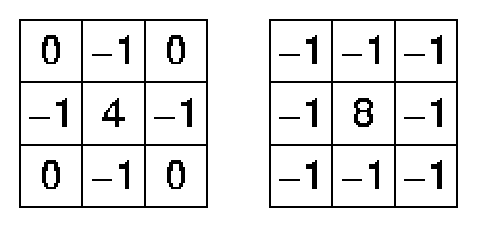
\includegraphics[scale=1]{Slike/laplace}
    \caption{Laplace filter \cite{laplace}}
\end{figure}

\begin{figure}[htbp]
    \centering
    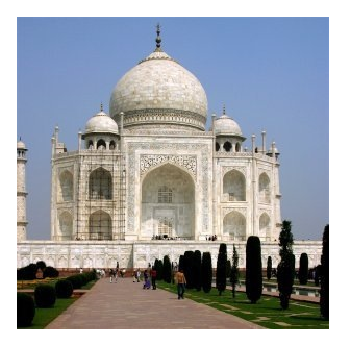
\includegraphics[scale=0.75]{Slike/taj_orig}
    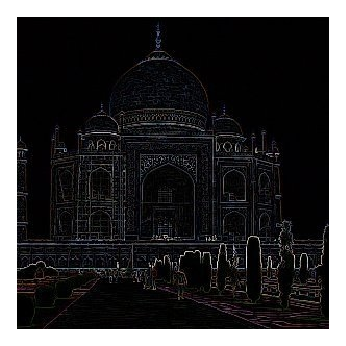
\includegraphics[scale=0.75]{Slike/edge-taj-laplace}
    \caption{Primjer djelovanja Laplace filtra na sliku \cite{laplaceexample}}
\end{figure}

\pagebreak

Konvolucijskim prozorom se prolazi kroz cijelu sliku, sumirajući težinski pikselne vrijednosti, te na izlazu dobijemo obrađenu sliku. Primjer djelovanja Laplace filtra dan je na slici 2.9.\par

Upravo ideja da se koriste konvolucijski operatori s filtrima koji su naučeni, a ne predodređeni, omogućile su neuronskim mrežama izrazit uspjeh u polju računalnog vida. Pri obradi slike to je od iznimne važnosti jer se postiže lokalna osjetljivost i dijeljenje parametara, odnosno model sam nauči mapiranje iz slike u prostor značajki koji je kasnije povezan na potpuno povezani sloj najčešće, ili nekakav drugi klasifikator. \par

Korištenje konvolucijskih slojeva omogućava slojevitiju mrežu, pošto su parametri dijeljeni, problem naglog rasta broja parametara sa slojevitošću je manji nego kod potpuno povezanih slojeva višeslojnog perceptrona. Stoga se konvolucijski slojevi bliže ulaznoj slici najčešće fokusiraju na detekciju značajki niske razine poput rubova i linija, dok kasniji konvolucijski slojevi modeliraju značajke viših razina poput razumijevanja scene i objekata.

\subsection{Slojevi sažimanja}
Uz konvolucijske slojeve često se u arhitekturama konvolucijskih neuronskih mreža mogu pronaći i slojevi sažimanja. Najčešće korišten operator je sažimanje po maksimalnom odzivu, no postoji sažimanje po minimalnom i prosječnom odzivu. Slojevi sažimanja općenito primaju sliku te zatim po regijama slike primjenjuju odabrani operator. Postižu smanjenje dimenzionalnosti, posljedično i smanjenje broja parametara modela što spriječava prenaučenost.

\begin{figure}[htbp]
    \centering
    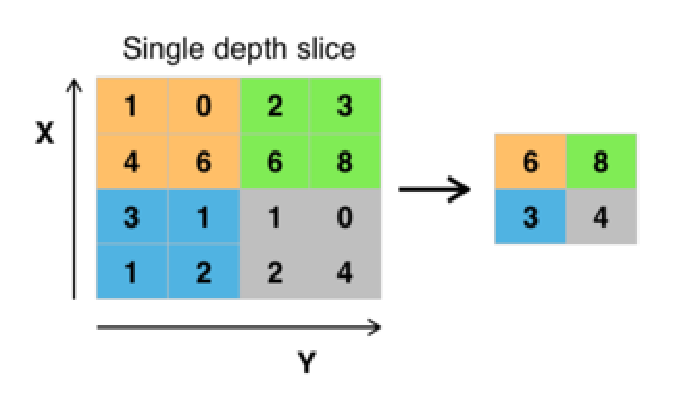
\includegraphics[scale=1]{Slike/Max_pooling}
    \caption{Primjer sažimanja po maksimalnom odzivu \cite{maxpoolexample}}
\end{figure}

\subsection{Arhitektura konvolucijskih neuronskih mreža}
Konvolucijske neuronske mreže primaju 2D ulaze poput slike, provlače ih kroz prvi konvolucijski sloj, nakon što se dobije prva mapa značajki, neuroni konvolucijskog sloja primjenjuju aktivacijske funkcije te se nakon toga vrši sloj sažimanja. Taj proces se ponavlja ovisno o tome koliko arhitektura mreže ima konvolucijskih slojeva. Izlaz zadnjeg konvolucijskog sloja je također mapa značajki koja se zatim "izravna" te se predaje potpuno povezanim slojevima. \par

\begin{figure}[htbp]
    \centering
    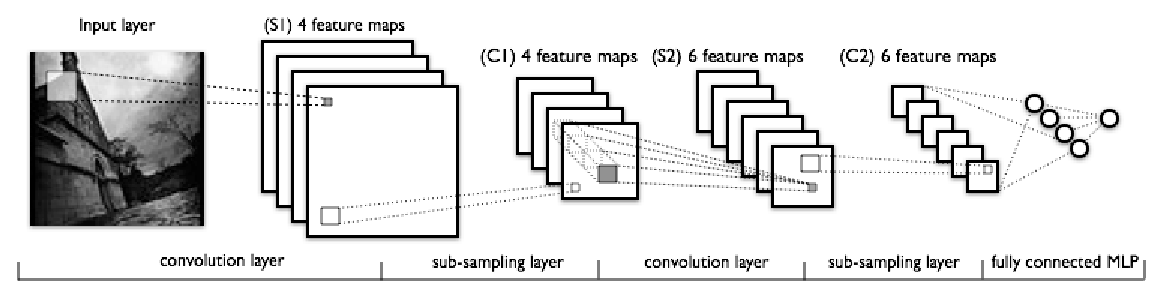
\includegraphics[scale=0.75]{Slike/mylenet}
    \caption{Primjer arhitekture konvolucijske neuronske mreže \cite{mylenet}}
\end{figure}

Predložena su i pojednostavljenja u arhitekturama konvolucijskih mreža \cite{striving}. Predloženo je izbacivanje slojeva sažimanja te proširenje koraka konvolucijskih filtara. Moderni duboki modeli za analizu slike izbjegavaju korištenje potpuno povezanih slojeva \cite{fullyconv}. \par

U zadnje vrijeme počeo se koristi pojam prijenosa učenja (engl. \textit{transfer learning}). Odnosi se na to da se mreža naučena nad jednim skupom podataka primjenjuje i nad drugim skupovima podataka. Često samo zahtijeva modifikacije nad posljednjim klasifikacijskim slojem jer se skupovi podataka razlikuju u broju klasa. Proces treniranja je isti, no praksa je pokazala da značajke naučene na problemu s velikim brojem primjera za učenje služe bolje od učenja nove mreže s incijaliziranim težinama. Stoga nije ni čudo da do sada već postoji par standardnih modela koji su unaprijed naučeni za klasifikaciju na ImageNetu \cite{imagenet}, koje se dalje prilagođavaju nad ostalim skupovima podataka. Najčešće se koristi kada za ciljani zadatak postoji puno manje primjera za učenje nego što je to slučaj od osnovnog zadatka za koji je mreža naučena.

\pagebreak

\section{Grupna normalizacija}
Grupna (engl. \textit{batch}) normalizacija je suvremena metoda za efektivno učenje neuronskih mreža \cite{batchnorm}. Motivacija je parametrizirano normalizirati ulaze u svaki sloj neuronske mreže pošto se distribucije ulaza u slojeve mijenjaju kroz treniranje. Gore navedeni problem povlači i druge probleme poput opreznog postavljanja stope učenja te inicijalizacije parametara mreže. Grupna normalizacija do neke mjere eliminira te probleme. Grupe se normaliziraju po sljedećim izrazima:

\begin{equation}
\mu_B = \frac{1}{m}\sum_{i=1}^m x_i
\end{equation}

\begin{equation}
\sigma_B^2 = \frac{1}{m}\sum_{i=1}^m (x_i - \mu_B)^2
\end{equation}

\begin{equation}
\hat{x_i} = \frac{x_i - \mu_B}{\sqrt{\sigma_B^2 + \epsilon}}
\end{equation}

\begin{equation}
y_i = \gamma \hat{x_i} + \beta
\end{equation}

Jednadžba 2.38 računa prosječnu vrijednost grupe, jednadžba 2.39 računa varijancu grupe. Koristeći oboje, podaci iz grupe se normaliziraju na prosječnu vrijednost 0 s varijancom 1 s izrazom 2.40. Izraz 2.41 nudi 2 parametra, $\gamma$ i $\beta$ koji mogu skalirati i pomaknuti distribuciju. To su optimizirajući parametri, odnosno optimizacijski postupci traže idealne $\gamma$ i $\beta$ za svaki sloj. $y_i$ predstavlja izlaz iz grupe normalizacije, odnosno transformirani ulaz. \par

Metoda se ispostavila od značajne važnosti jer ulazi kasnijih slojeva više ne ovise o magnitudama prijašnjih slojeva pošto se vrši parametrizirana normalizacija. Model sam nauči parametre grupne normalizacije, odnosno skaliranje i pomak normalno distribuiranih ulaza. Autori su eksperimentima pokazali da postupak dovodi do brže konvergencije i boljih rezultata, te se grupna normalizacija smatra neizostavnim dijelom većine modernih arhitektura dubokih neuronskih mreža.\par

Grupna normalizacija se primjenjuje na poseban način kod konvolucijskih slojeva neuronskih mreža. Za razliku od potpuno povezanih slojeva, gdje cijeli sloj dijeli parametre $\gamma$ i $\beta$, kod konvolucijskih slojeva oni su dijeljeni po mapama značajki \cite{convbatchnorm}. Dakle, neuroni unutar jedne mape značajki ne dijele samo težinske parametre, već i normalizacijske. To je potrebno radi očuvanja glavnog svojstva konvolucijskih neuronskih mreža, invarijantnosti na translaciju.



\chapter{Generativne suparničke mreže}
Generativne suparničke mreže predstavljaju modele u kojima su suprotstavljene dvije neuronske mreže, generator i diskriminator \cite{GAN}. Zadatak generatora je modelirati distribuciju ulaznih podataka, a zadatak diskriminatora je odrediti da li podatak potječe iz stvarnog skupa ili je generiran generatorom. Diskriminator minimizira binarnu klasifikacijsku funkciju pogreške (da li je podatak na ulazu stvaran ili generiran), dok generator maksimizira grešku diskriminatora za generirane podatke. Model se uči nenadziranim učenje, odnosno nisu mu potrebni označeni podaci. Pošto su generator i diskriminator neuronske mreže, uče se algoritmom unazadne propagacije te nisu potrebne vjerojatnosne estimacije podataka kao kod drugih generativnih modela. \par

Generator je neuronska mreža koja na ulazu prima šum (najčešće uniformne ili normalne distribucije), provodi šum kroz skrivene slojeve, te na izlazu daje sliku. Vektor uzorkovan iz šuma najčešće označavamo s $z$, dok vjerojatnosnu distribuciju šuma označavamo s $p_z$. Zadatak generatora je modelirati vjerojatnosnu distribuciju $p_g$, da bude što sličnija distribuciji stvarnih podataka $p_ {data}$. Globalno, generator se može interpretirati kao diferencijabilna funkcija $G(z; \theta_g)$, koja prima vektor šuma $z$, te parametrima $\theta_g$ definira preslikavanje šuma u podatkovni prostor. \par

Diskriminator je neuronska mreža koja na ulazu prima stvaran ili generiran podatak, provodi ga kroz skrivene slojeve te na izlazu daje skalarnu vrijednost, odnosno vjerojatnost pripadanja ulaza stvarnim podacima. Diskriminator predstavlja diferencijabilnu funkciju $D(x, \theta_d)$, koja prima vektor podatka $x$ te parametrima $\theta_d$ definira klasifikaciju, odnosno da li je podatak stvaran ili generiran. \par

Generator i diskriminator igraju minimax igru sa sljedećom kriterijskom funkcijom:

\begin{equation}
\stackunder{min}{\textbf{G}}\hspace{0.1cm}\stackunder{max}{\textbf{D}}\hspace{0.1cm} V(D,G) = \mathbb{E}_{x \thicksim p_{data}(x)}[\log D(x)] + \mathbb{E}_{z \thicksim p_z(z)}[\log (1 - D(G(z))]
\end{equation}

\pagebreak

Kroz jednadžbu (3.1) zadan je maksimizacijski izraz za diskriminator, iz izraza je također očigledan i minimizacijski izraz generatora, odnosno generator minimizira $\log (1 - D(G(z))$. Praksa je pokazala da minimiziranje tog izraza daje slabije gradijente na početku, te se savjetuje maksimizacija $\log D(G(z)$ \cite{GAN}. Algoritam generativne suparničke mreže glasi:\\

\begin{algorithm}[H]
 \For{number of training iterations}{
  \For{ksteps}{
  Sample minibatch of $m$ noise samples $\{z^{(1)}, ... , z^{(m)}\}$ from $p_z(z)$\\
  Sample minibatch of $m$ examples $\{x^{(1)}, ... , x^{(m)}\}$ from real data \\
  Update the discriminator by ascending its stochastic gradient:
  \begin{equation}
  \nabla_{\theta_d}\frac{1}{m}\sum_{i=1}^m \left[\log D(x^{(i)}) + \log(1 - D(G(z^{(i)})))\right]
  \end{equation}
   }
  Sample minibatch of $m$ noise samples $\{z^{(1)}, ... , z^{(m)}\}$ from $p_z(z)$\\
  Update the generator by ascending its stochastic gradient:
    \begin{equation}
  \nabla_{\theta_g}\frac{1}{m}\sum_{i=1}^m \log D(G(z^{(i)}))
  \end{equation}
 }
 \caption{GAN}
\end{algorithm}

Model generativnih suparničkih mreža podrazumijeva treniranje diskriminatora do optimalnosti. Algoritam radi s numeričkom aproksimacijom gdje se diskriminator trenira određen broj koraka, jer bi inače model bio vremenski preskup. Praksa je pokazala da je dovoljno trenirati diskriminator jednom, a nekad generator više puta jer model pati od nestabilnosti pošto diskriminator prebrzo nauči razlikovati podatke, no o tome više u sljedećem poglavlju. Slika 3.1 ilustrira generativnu suparničku mrežu.

\begin{figure}[htbp]
    \centering
    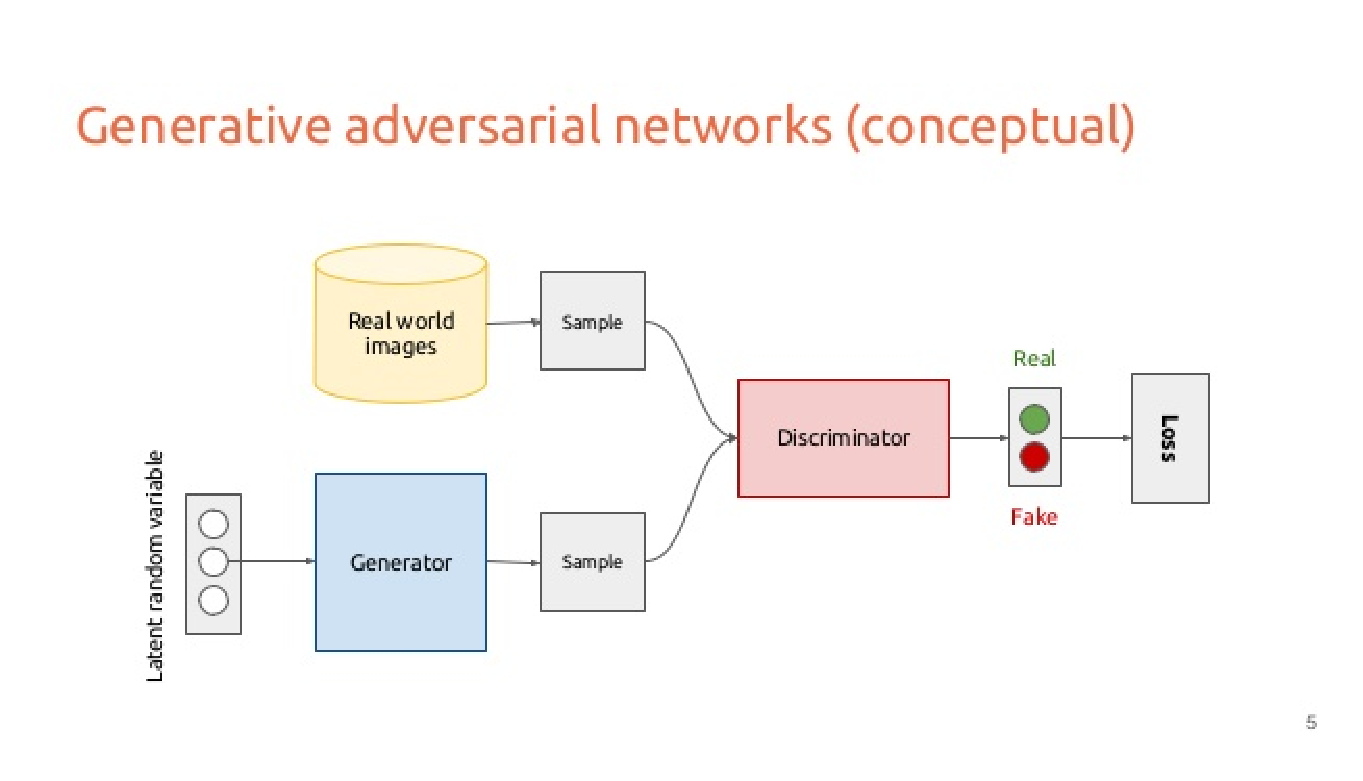
\includegraphics[scale=0.7]{Slike/gan}
    \caption{Generativna suparnička mreža \cite{gansketch}}
\end{figure}

\pagebreak

\section{Globalni optimum modela}
Globalni optimum modela se dobije kada $p_g = p_{data}$. Slijedi i dokaz za tu tvrdnju. Prvo izvodimo optimalan diskriminator za bilo koji generator.

\begin{prop}
Za fiksiran generator, optimalan diskriminator glasi:
\begin{equation}
D_G^*(x) = \frac{p_{data}(x)}{p_{data}(x) + p_g(x)}
\end{equation}
\begin{proof}
Jednadžba (3.1) daje kriterij koji diskriminator optimizira bez obzira na generator.
\begin{gather}
V(G,D) = \int_x p_{data}(x) \log D(x)dx + \int_z p_{z}(z) \log (1 - D(G(z))dz \\ 
\nonumber = \int_x (p_{data}(x) \log D(x) + p_{g}(x) \log (1 - D(x)))dx
\end{gather}
Cilj je pronaći optimalan D(x). Deriviranjem funkcije pod integralom te pronalaženjem optimalnog D(x) optimizirali smo i izraz V pošto optimalni D maksimizira V u svakoj točki. Radi jednostavnosti notacije, gornji podintegralni izraz svest ćemo na:
\begin{equation}
f(y) = a\log y + b\log (1-y)
\end{equation}
gdje je $a=p_{data}(x)$, $b=p_g(x)$, $y=D(x)$.
\begin{equation}
f'(y) = \frac{a}{y} - \frac{b}{1-y}
\end{equation}
Za dobit ekstrem funkcije prvu derivaciju izjednačimo s 0.
\begin{gather}
\frac{a}{y} - \frac{b}{1-y} = 0 \\
\nonumber\frac{a}{y} = \frac{b}{1-y} \\
\nonumber a - ay = by \\
\nonumber a = ay + by \\
\nonumber a = y(a+b) \\
\nonumber y = \frac{a}{a+b}
\end{gather}
Gornji izraz je ekstrem funkcije, sada treba provjeriti vrijednost druge derivacije funkcije u toj točki, ukoliko je negativna radi se o maksimumu, a maksimum je u ovom slučaju optimum.
\begin{gather}
f''(y) = - \frac{a}{y^2} - \frac{b}{(1-y)^2} \\
\nonumber f''\left(\frac{a}{a+b}\right) = - \frac{a}{\left(\frac{a}{a+b}\right)^2} - \frac{b}{(1-\frac{a}{a+b})^2}
\end{gather}
Pošto se radi s vjerojatnostima koje su definirane na intervalu [0, 1], gornji izraz je uvijek negativan (osim kada $a=b=0$, ali taj slučaj nema smisla razmatrati), te smo dobili da je $\frac{a}{a+b}$ maksimum tražene funkcije, odnosno da vrijedi:
\begin{equation}
D_G^*(x) = \frac{p_{data}(x)}{p_{data}(x) + p_g(x)}
\end{equation}
\end{proof}
\end{prop}
Nakon pronalaska optimalnog diskriminatora, slijedi teorem koji potvrđuje da se globalni optimum minimax igre, odnosno kriterijske funkcije nalazi u $p_g = p_{data}$
\begin{theorem}
Globalni minimum kriterija $C(G)$ je postignut ako i samo ako $p_g = p_{data}$ te u toj točki on iznosi $\log \frac{1}{4}$.
\begin{proof}
\begin{align}
C(G) &= \stackunder{max}{\textbf{D}} V(D,G) \\
\nonumber &= V(D^*,G) \\
\nonumber &= \mathbb{E}_{x \thicksim p_{data}(x)}[\log D^*(x)] + \mathbb{E}_{x \thicksim p_g(x)}[\log (1 - D^*(x)] \\
\nonumber &= \int_x p_{data}(x) \log D^*(x)dx + \int_x p_{g}(x) \log (1 - D^*(x))dx \\
\nonumber &= \int_x p_{data}(x) \log \left(\frac{p_{data}(x)}{p_{data}(x) + p_g(x)}\right)dx + \int_x p_g(x) \log \left(1 - \frac{p_{data}(x)}{p_{data}(x) + p_g(x)}\right)dx \\
\nonumber &= \int_x p_{data}(x) \log \left(\frac{p_{data}(x)}{p_{data}(x) + p_g(x)}\right)dx + \int_x p_g(x) \log \left(\frac{p_g(x)}{p_{data}(x) + p_g(x)}\right)dx \\
\nonumber &= \int_x p_{data}(x) \log \left(\frac{p_{data}(x)}{\frac{p_{data}(x) + p_g(x)}{2}}\right)dx - \int_x p_{data}(x)\log 2 dx \\
\nonumber &+ \int_x p_g(x) \log \left(\frac{p_g(x)}{\frac{p_{data}(x) + p_g(x)}{2}}\right)dx - \int_x p_g(x)\log 2 dx \\
\nonumber &= \int_x p_{data}(x) \log \left(\frac{p_{data}(x)}{\frac{p_{data}(x) + p_g(x)}{2}}\right)dx - \log 2 \\
\nonumber &+ \int_x p_g(x) \log \left(\frac{p_g(x)}{\frac{p_{data}(x) + p_g(x)}{2}}\right)dx - \log 2 \\
\nonumber &= KL\left(p_{data} \| \frac{p_{data} + p_g}{2}\right) + KL\left(p_g \| \frac{p_{data} + p_g}{2}\right) - 2\log2 \\
\nonumber &= -\log4 + 2JSD(p_{data} \| p_g) \\
\nonumber &= \log\frac{1}{4} + 2JSD(p_{data} \| p_g)
\end{align}
\end{proof}
\end{theorem}
Kada vrijedi $p_{data} = p_g$ tada je Jensen-Shannon divergencija jednaka nuli, te se dobije globalni minimum $\log\frac{1}{4}$. Tada generator savršeno replicira distribuciju stvarnih podataka. U svim ostalim slučajevima, Jensen-Shannon divergencija je veća od 0 stoga se distribucija $p_g$ ne nalazi u globalnom minimumu.

\pagebreak

\section{Duboke konvolucijske generativne suparničke mreže}
U generativnim suparničkim mrežama na početku poglavlja predviđeni su višeslojni perceptroni kao odabran model za generator i diskriminator. Duboke konvolucijske generativne suparničke mreže koriste konvolucijske arhitekture \cite{radford}. Primjena već poznatih i često korištenih dubokih arhitektura ne garantira uspješnost treniranja modela jer generativne suparničke mreže pate od degradacije treniranja u propast (pojava pri kojoj generator daje istu sliku za proizvoljan vektor šuma, ne učeći pritom modeliranje stvarnih slika) za velik broj arhitektura, te je pronalazak stabilnih arhitektura možda i najveći izazov pri njihovoj primjeni. Autori u gore spomenutom radu navode tri važna faktora pri modeliranju dubokih konvolucijskih generativnih suparničkih mreža. \par

Prvi faktor je korištenje konvolucijskiih mreža bez slojeva sažimanja, već korištenje konvolucija s korakom preko kojeg mreže uče prostorno povećanje ili sažimanje. Generator tako uči prostorno povećanje preko dekonvolucija s korakom, a diskriminator prostorno sažimanje preko konvolucija s korakom. Korak je hiperparametar modela, najčešći odabir je korak veličine 2 u obe dimenzije konvolucije.\par

Drugi faktor je izostavljanje potpuno povezanih slojeva. Generator uzima vektor šuma iz latentnog prostora, zatim koristi potpuno povezan sloj za postići određene dimenzije u skrivenom sloju, no taj sloj se preoblikuje u 4D tensor gdje jedna dimenzija odgovara veličini grupe, dvije dimenzije predstavljaju matricu veličine slike, a zadnja dimenzija je broj kanala u slici. Slojevi dekonvolucije se ponavljaju dok se ne dođe do traženih dimenzija. Kod diskriminatora, na ulaz se direktno primjenjuju konvolucijski slojevi do posljednjeg, koji se zatim "izravna" te predaje sigmoidalnom neuronu. \par

Treći faktor je korištenje grupne normalizacije što pridonosi stabilnijem treniranju ukupnog modela, te izbjegavanju degradacije treniranja u propast.
Grupna normalizacija se ne primjenjuje na ulaz u diskriminator, te na izlaz generatora jer se eksperimentalno pokazalo da to vodi nestabilnijem treniranju \cite{radford}. Također se savjetuje korištenje ReLU aktivacijska funkcija, te Leaky ReLU što predstavlja parametriziranu ReLU funkciju gdje je parametar $a \in <0,1>$. \par

\begin{figure}[htbp]
    \centering
    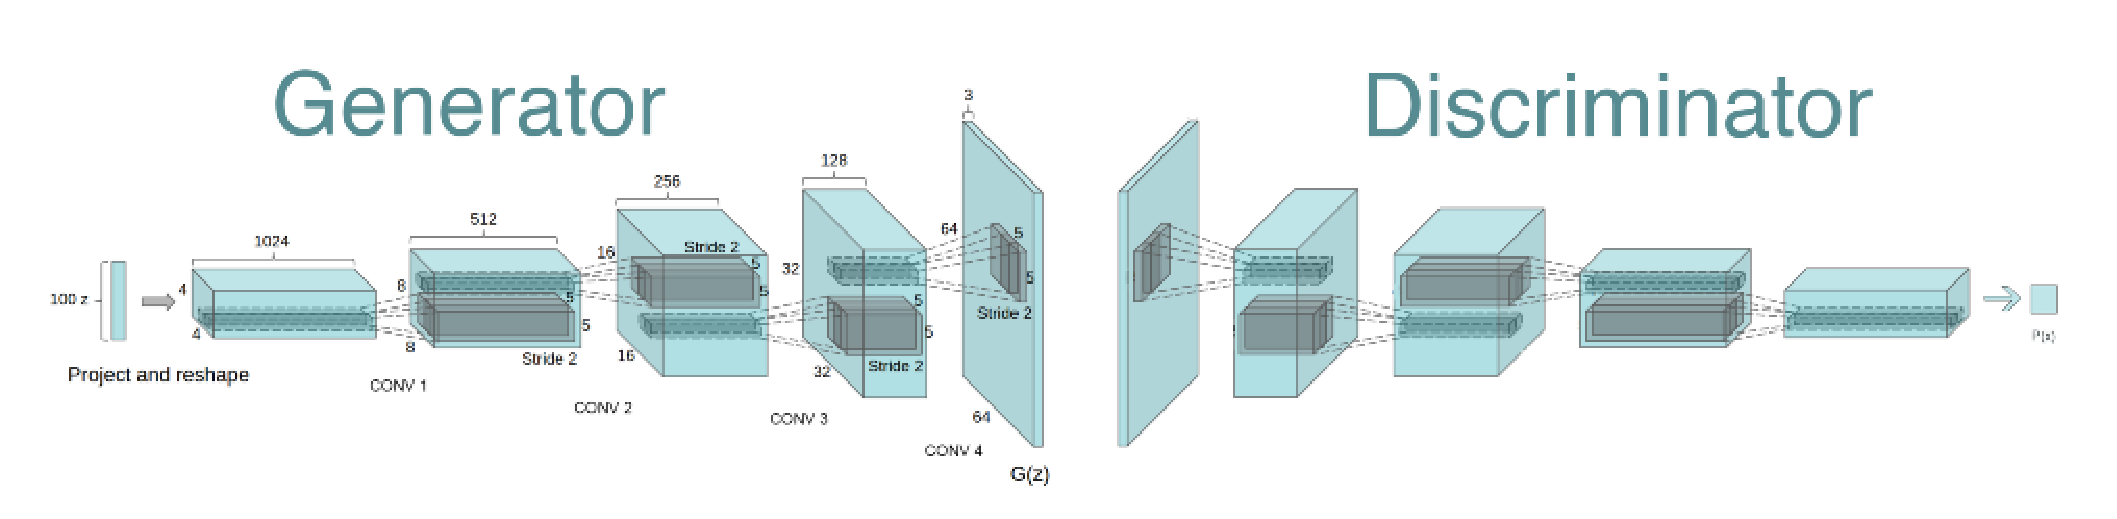
\includegraphics[scale=0.4]{Slike/dcgan}
    \caption{Duboka konvolucijska generativna suparnička mreža \cite{dcgan}}
\end{figure}

\section{Klasifikatorska generativna suparnička mreža}
Gore spomenuti modeli uče isključivo nenadzirano, odnosno nisu im potrebni označeni primjeri. Klasifikatorska generativna suparnička mreža zahtijeva označene primjere za učenje, te istovremeno diskriminator uči klasifikaciju primjera po danim oznamaka, kao i binarnu klasifikaciju da li je podatak stvaran ili generiran \cite{acgan}. \par

Generatoru generira vektor šuma na koji doda oznaku koja mu je proslijeđena, stoga generator uči generirati podatke po klasi što mu znatno olakšava posao. Diskriminator ima 2 gubitka, gubitak po uzorkovanju te po klasifikaciji, model je usporediv s pravim nadziranim klasifikatorima, no u praksi se nije pokazao boljim. Obe tvrdnje će biti pokazane u slijedećem poglavlju. \par

\begin{figure}[htbp]
    \centering
    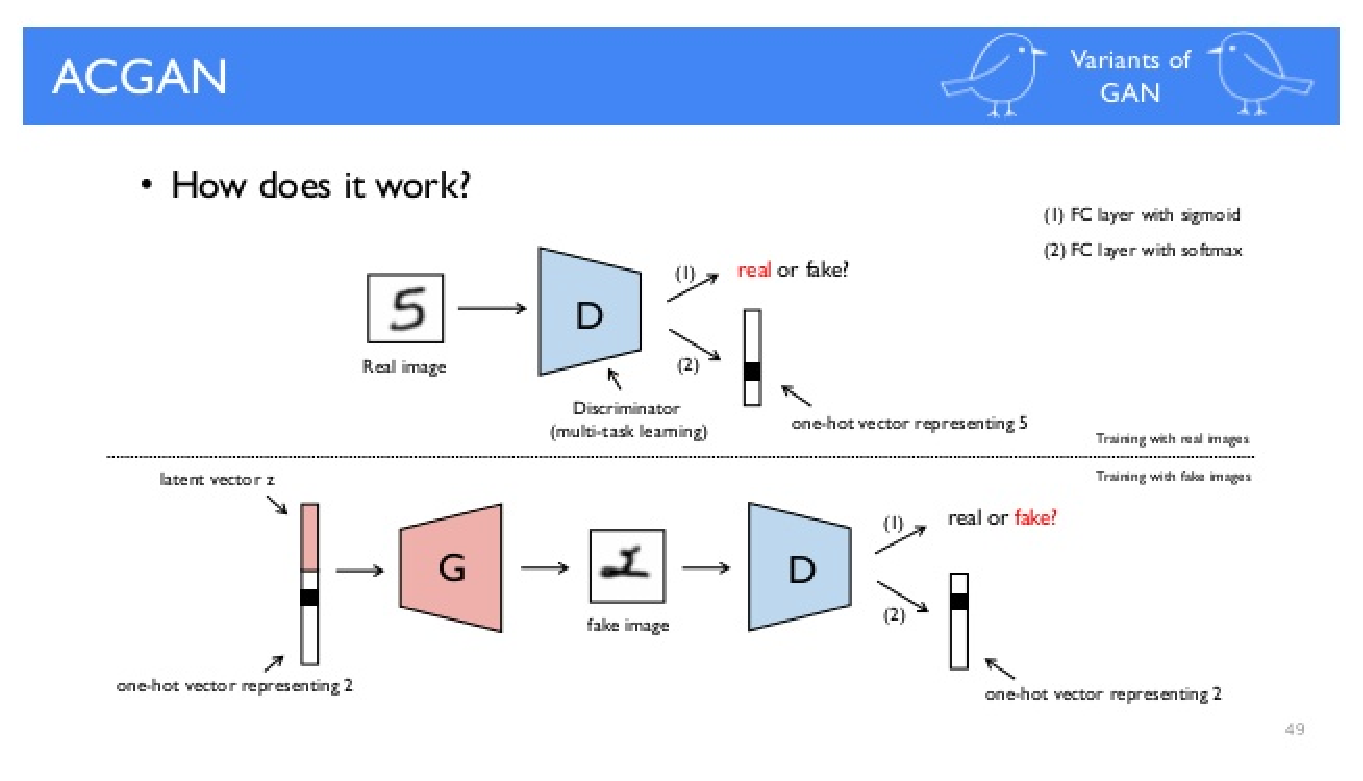
\includegraphics[scale=0.6]{Slike/acgan}
    \caption{Klasifikatorska generativna suparnička mreža \cite{acgansketch}}
\end{figure}

Funkcije izglednosti izgledaju:
\begin{gather}
L_S = \mathbb{E}[\log P(S = real | X_{real})] + \mathbb{E}[\log P(S = fake | X_{fake})] \\
\nonumber L_C = \mathbb{E}[\log P(C = c | X_{real})] + \mathbb{E}[\log P(C = c | X_{fake})]
\end{gather}
gdje $L_S$ predstavlja izglednost uzorkovanja diskriminatora, a $L_C$ klasifikacijsku izglednost. Diskriminator maksimizira vrijednost $L_S + L_C$ dok generator maksimizira $L_C - L_S$.

\chapter{Implementacija i rezultati}
Eksperimenti su provedeni na računalu s operacijskim sustavom Ubuntu 16.04 LTS, procesorom Intel i5-6600, grafičkom karticom GTX1060 6GB te 16GB RAMa. Za programsku implementaciju korišten je Tensorflow \cite{tensorflow} te Python3. Za usporedbu i pomoć autor se poslužio implementacijama dostupnim na webu \cite{wiseodd}\cite{carpedm}.

\section{Skupovi podataka}
U ovoj sekciji opisani su skupovi podataka na kojima se model trenirao. \par

\subsection{MNIST}
Za većinu eksperimenata korištena je baza rukom pisanih znakova MNIST \cite{mnist}. Sastoji se od 55000 primjera za učenje, 5000 za validaciju, te 10000 za testiranje. Slike su dimenzija 28x28, a oznake dolaze kao vektor dimenzija 1x10 gdje broj jedan označava znamenku koju slika predstavlja. Slika 4.1 ilustrira neke od primjera iz skupa podataka. Slika 4.2 prikazuje primjere iz baze.

\begin{figure}[H]
    \centering
    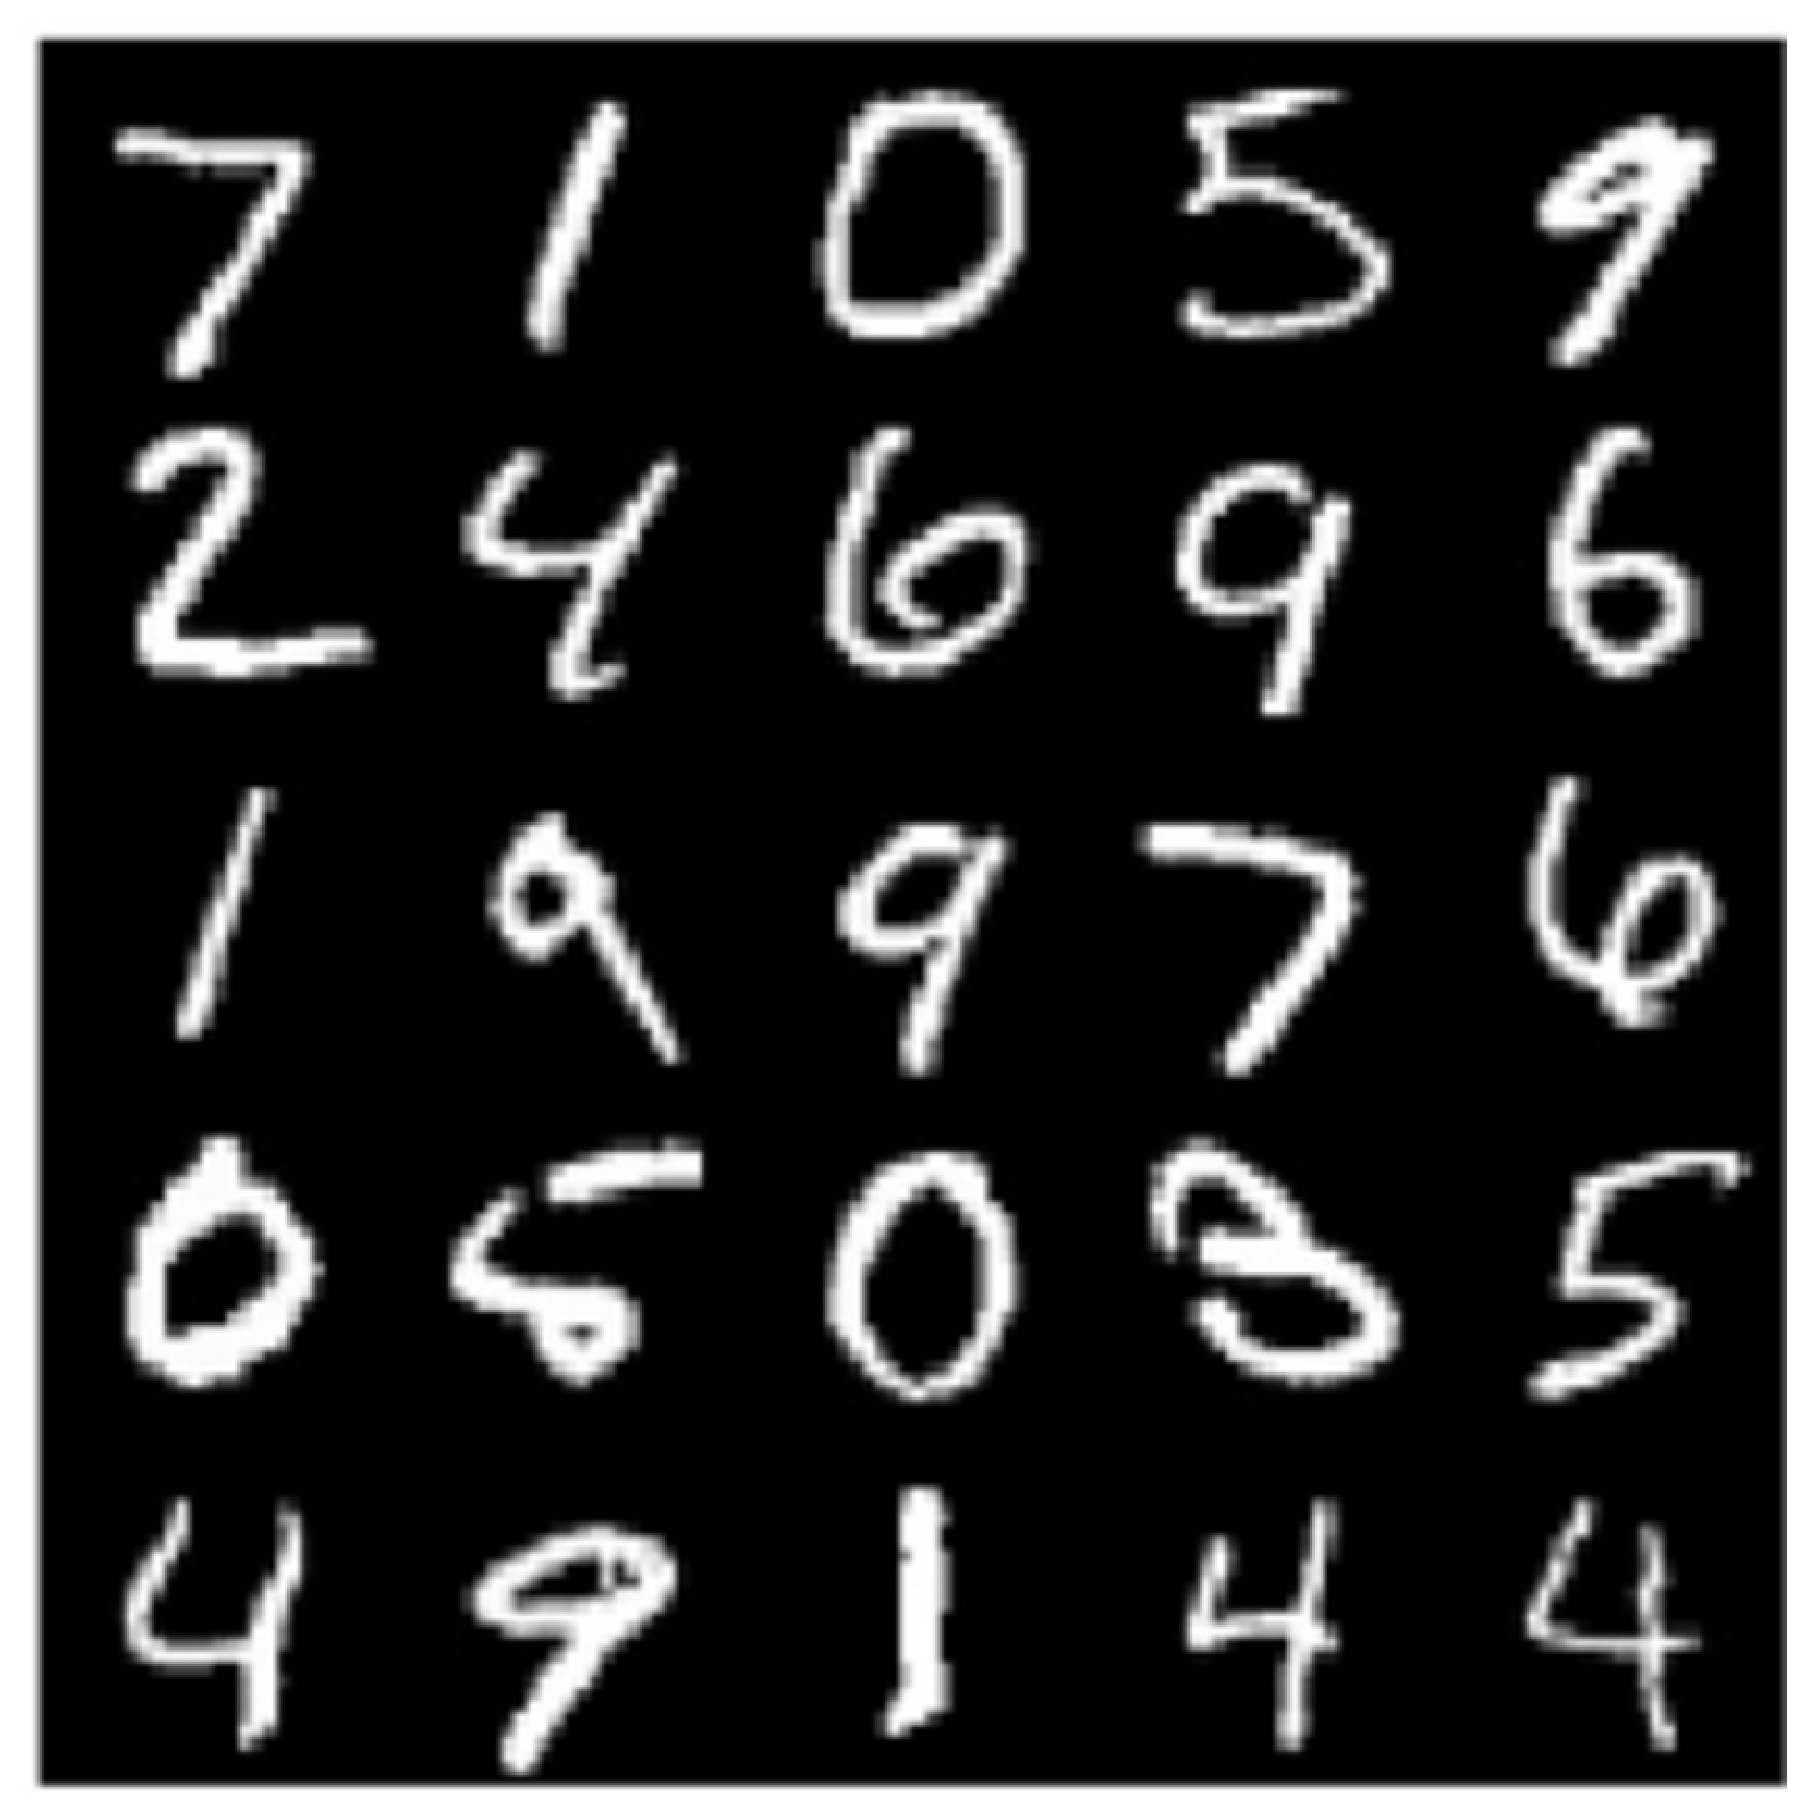
\includegraphics[scale=0.25]{Slike/mnist}
    \caption{Primjeri MNIST znakova}
\end{figure}

\subsection{FM3}
FM3 je baza slika nadograđena na FM2 koja je pobliže opisana u radu \cite{sikiric}. Sastoji se od 6442 slike u boji iz prometa podijeljene u 8 klasa. Za učenje je predviđeno 3222 primjera, a za testiranje 3220 primjera. Slike su rezolucije 640x480x3 nastale u prometu, iz postavljene kamere na autu dok se vozio cestama. Pretprocesiranje se sastojalo od svođenja slike na kvadratni format 480x480x3 tako što je oduzeto 80 piksela s lijeve i desne strane, zatim preoblikovanje u sliku dimenzija 32x32x3 koja se dalje prosljeđivala modelu.

\begin{figure}[H]
\begin{center}

\includegraphics[width=.33\textwidth]{000001}
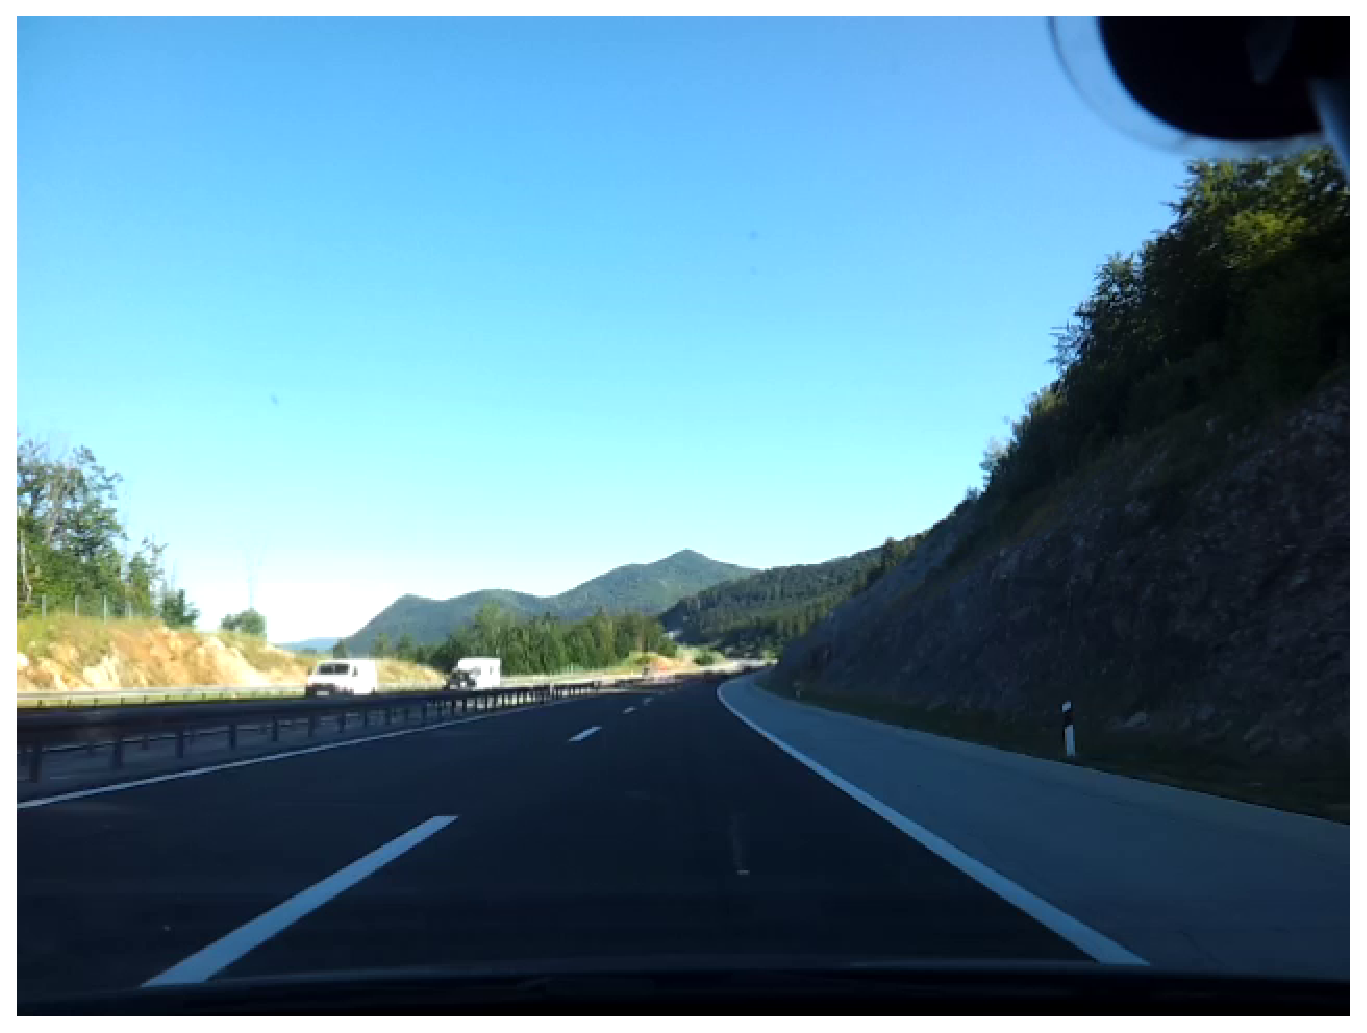
\includegraphics[width=.33\textwidth]{000855}

\includegraphics[width=.33\textwidth]{003935}

\includegraphics[width=.33\textwidth]{006437}
\end{center}
\caption{Primjeri iz baze slika FM3}
\end{figure}

\section{Generativna suparnička mreža}
Generativna suparnička mreža zamišljena je pomoću dvaju višeslojnih perceptrona, jedan u ulozi diskriminatora, drugi u ulozi generatora. Početak modela predstavlja uzorkovanje iz šuma. Za veličinu vektora šuma odredili smo 100, odnosno vektor je veličine 1x100. Uzorkujemo ga iz distribucije $\mathcal{N}(0,1)$. Prvi potpuno povezani sloj je veličine 100x200, te on preslikava šum na ulazu u skriveni sloj. Izlazni sloj je potpuno povezani sloj veličine 200x784 (odgovara dimenzijama slike 28x28). Skriveni sloj koristi ReLU aktivacijsku funkciju, izlazni sloj koristi sigmoidu. Diskriminator dobije ulaz veličine 784 (kada se "izravna" slika). Prvi skriveni sloj ima dimenzije 784x200 te koristi ReLU aktivacijsku funkciju, izlazni sloj je veličine 200x1 te koristi sigmoidalni neuron koji određuje vjerojatnost da je ulazni podatak stvaran. Za optimizaciju parametara diskriminatora koristi se stohastički gradijentni spust s stopom učenja 0.01, za optimizaciju parametara generatora koristi se Adam optimizator s predefiniranim parametrima. Težine se inicijaliziraju normalnom distribucijom s srednjom vrijednosti 0, a standardnom devijacijom 0.01, te se odbijaju sve generirane težine koje odstupaju za više od dvije standardne devijacije (\textit{tensorflow.truncated\_normal}), težine pristranosti se postavljaju na 0.1.\par

Odabrana veličina grupe primjera je 500, te postupak treniranja traje 100000 iteracija, crtajući nasumične uzorke koji se preslikavaju iz latentnog u podatkovni prostor svakih 5000 iteracija. Slika 4.3 ilustrira proces učenja generatora. Slika 4.4 prikazuje gubitke diskriminatora i generatora. U idealnom slučaju gubitak generatora bi trebao iznositi $log 2 \approx 0.3$, tada bi gubitak diskriminatora bio $log 4 \approx 0.6$. No, radi se o jednostavnom modelu, te ne možemo očekivati da on u potpunosti modelira stvarnu distribuciju podataka. Diskriminator i generator se treniraju jednom po iteraciji. Eksperimenti s više parametara i slojeva višeslojnog perceptrona vrlo lako mogu propasti radi nestabilnosti arhitektura. 


\begin{figure}[H]
\begin{center}
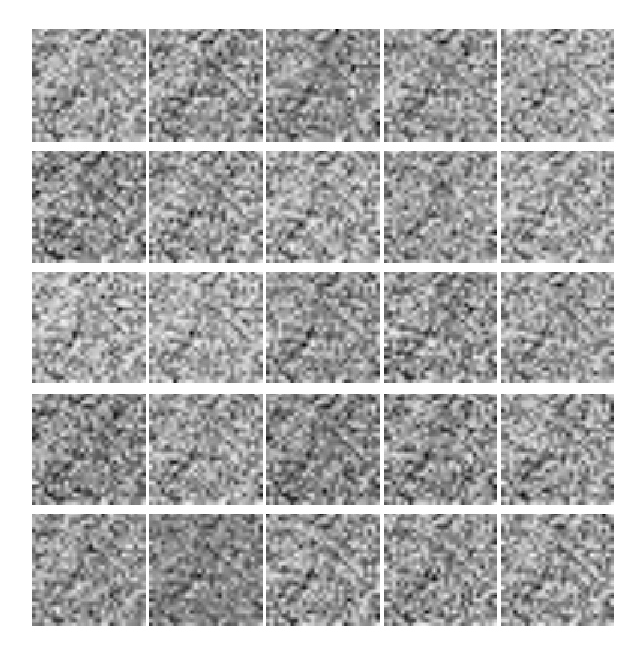
\includegraphics[width=.33\textwidth]{GAN000}
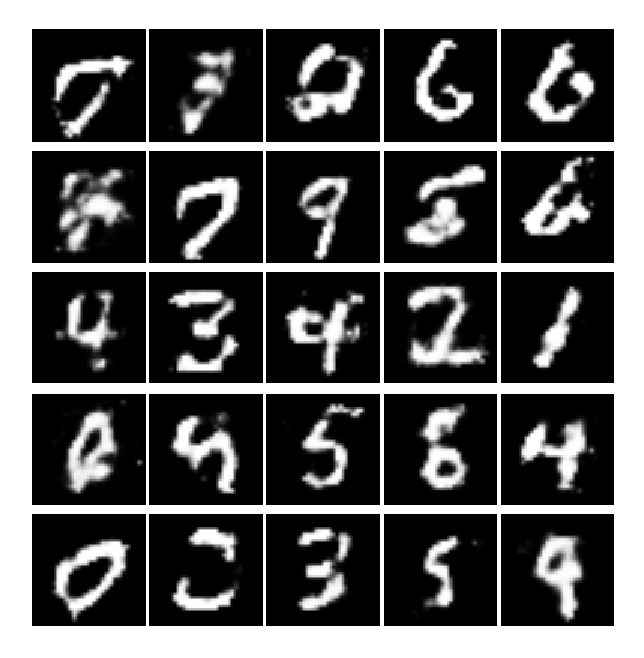
\includegraphics[width=.33\textwidth]{GAN005}
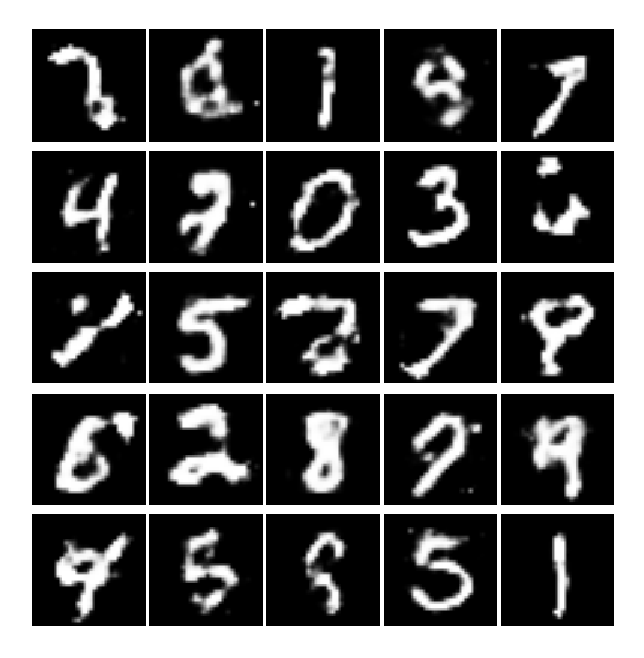
\includegraphics[width=.33\textwidth]{GAN010}
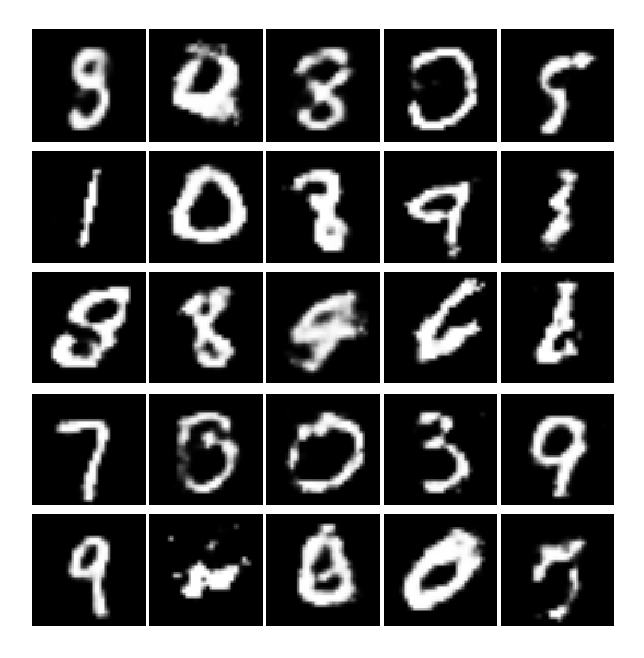
\includegraphics[width=.33\textwidth]{GAN020}
\end{center}
\caption{Uzorci nakon 0 (gore-lijevo), 25000 (gore-desno), 50000 (dolje-lijevo), 100000 (dolje-desno) iteracija}
\end{figure}

\begin{figure}[H]
\begin{center}
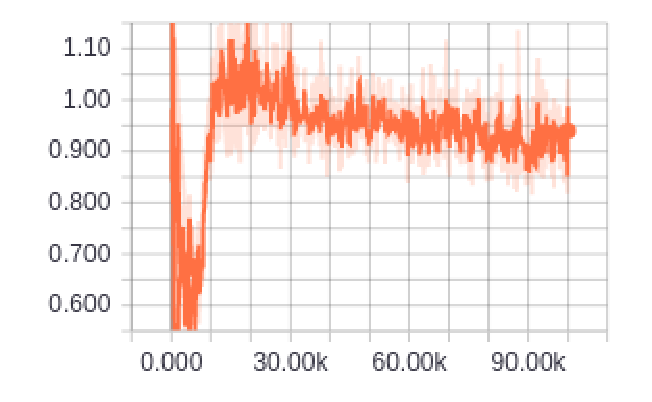
\includegraphics[width=.4\textwidth]{GANdiscloss}
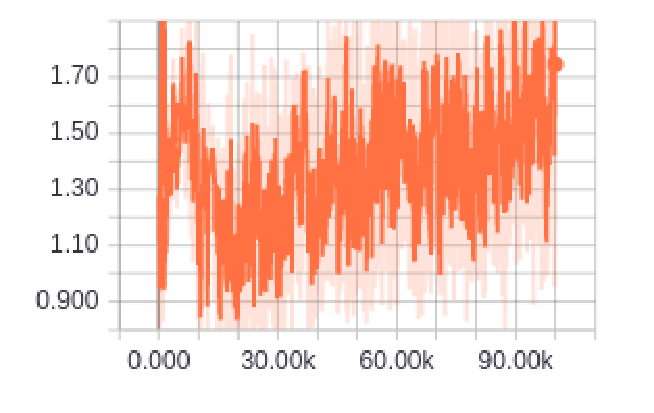
\includegraphics[width=.4\textwidth]{GANgenloss}
\end{center}
\caption{Gubitak diskriminatora (lijevo) i generatora (desno)}
\end{figure}

\pagebreak

\section{Duboke konvolucijske generativne suparničke mreže}
U svrhu dokaza da \cite{radford} vodi ka stabilnijem treniranju različitih arhitektura, implementirane su 4 modela s različitim generatorima. Prva 3 modela se razlikuju po broju potpuno povezanih slojeva na početku (broj potpuno povezanih slojeva ide od 1 do 3), te sva 3 imaju 2 dekonvolucijska, dok četvrti ima samo 1 potpuno povezan sloj i 4 dekonvolucijska sloja. Fokus će biti na arhitekturama 1 i 4. \par

Sve varijable su inicijalizirane s \textit{tensorflow.truncated\_normal} i standardnom devijacijom 0.02, težine pristranosti se postavljaju na 0.1. Za treniranje se koristi Adam optimizator kojem je stopa učenja postavljena na 0.0002, te $\beta_1$ parametar na 0.5. Veličina grupe iznosi 64, a postupak treniranja traje 100000 iteracija. Vektor šuma se ovdje uzorkuje iz $\mathcal{U}(-1,1)$. Važna napomena je da se za svako treniranje diskriminatora, generator trenira dvaput.\par

Generator prvog modela uzorkuje vektor šuma veličine 1x100 te je spojen na potpuno povezan sloj veličine 100x6272. Taj sloj se zatim preoblikuje u 7x7x128 gdje 7x7 predstavlja sliku koju generator povećava, a 128 broj kanala te slike. Sada slijedi dekonvolucijski sloj s pomakom 2 u obe dimenzije te dozvoljenim nadopunjavanjem. Dekonvolucijski sloj se sastoji od 7x7x128 filtara koji sliku na ulazu veličine 7x7x128, pretvore u sliku veličine 14x14x128. Idući dekonvolucijski sloj rezultira slikom dimenzija 28x28, njegov dekonvolucijski filtar je veličine 14x14x1. Grupna normalizacija se primjenjuje svugdje osim u zadnjem dekonvolucijskom sloju, aktivacijske funkcije su u svim slojevima ReLU, osim u zadnjem gdje se primjenjuje simgoidalna funkcija. \par

Generator četvrtog modela uzorkuje šum na isti način. Njegov potpuno povezani sloj je veličine 100x2048 koji se zatim preoblikuje u tenzor dimenzija 2x2x512. Dekonvolucijski filtri koriste nadopunjavanje te korak veličine 2. Prvi dekonvolucijski filtar je veličine 2x2x256, što znači da rezultira tenzorom 4x4x256. Drugi dekonvolucijski filtar je veličine 4x4x128, njegov izlaz je tenzor veličine 7x7x128. Treći dekonvolucijski filtar je veličine 7x7x64, njegov rezultat je tenzor veličine 14x14x64. Posljednji dekonvolucijski filtar je veličine 14x14x1 te je njegov rezultat slika dimenzija 28x28. Svi slojevi osim posljednjeg primjenjuju grupnu normalizaciju i ReLU, posljednji sloj koristi sigmoidalnu funkciju i nema grupnu normalizaciju. Generator četvrtog modela je nešto većeg kapaciteta od generatora prvog modela, te koristi više dekonvolucijskih slojeva stoga će bit zanimljivo usporediti dinamiku učenja oba modela. \par

Diskriminator sva 4 modela je isti. Ulaz mu je slika dimenzija 28x28. Prvi konvolucijski sloj je veličine 5x5x16, s korakom 2 i nadopunjavanjem, što znači da mu je izlazni tenzor veličine 14x14x16. Drugi konvolucijski sloj je veličine 5x5x32, s korakom 2 i nadopunjavanjem što znači da mu rezultira tenzorom 7x7x32. Treći konvolucijski sloj je veličine 5x5x64, s korakom 2 i nadopunjavanjem, izlaz mu je veličine 4x4x64. Posljednji konvolucijski sloj je veličine 5x5x128, s korakom 2 i nadopunjavanjem što znači da je njegov izlaz tenzor dimenzija 2x2x128. Taj tenzor se zatim izravna da bude sloj veličine 1x512 te se proslijedi sigmoidalnom neuronu koji određuje pripadnost podatka. Svi konvolucijski slojevi koriste \textit{leakyReLU} aktivacijsku funkciju, to je parametrizirana ReLU funkcija s parametrom $a=0.2$ u ovom slučaju. Također koriste grupnu normalizaciju. \par

Slika 4.5 prikazuje generirane slike u određenim iteracijama, slika 4.6 prikazuje gubitke generatora i diskriminatora kroz iteracije za prvi model. Ponašanjem prikazanih gubitaka, da se naslutiti da generator nije dovoljnog kapaciteta naspram diskriminatora, no svejedno nauči modelirati distribuciju stvarnih podataka do neke mjere. \par

\begin{figure}[H]
\begin{center}
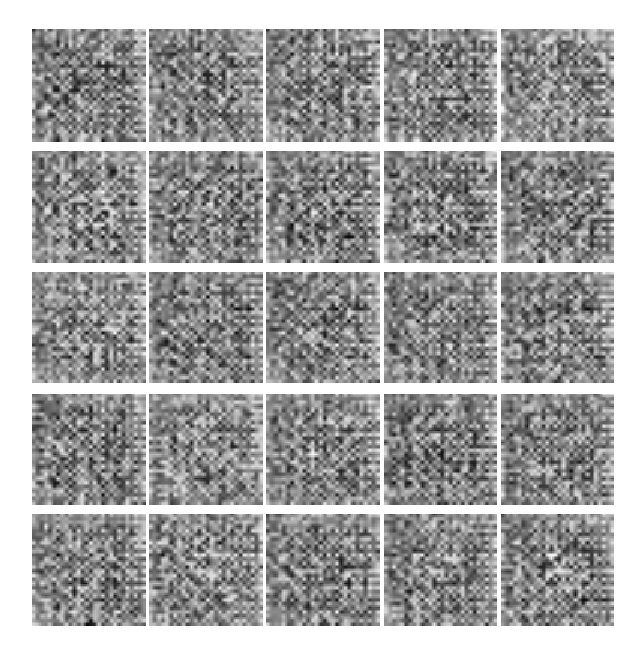
\includegraphics[width=.33\textwidth]{dcganmini000}
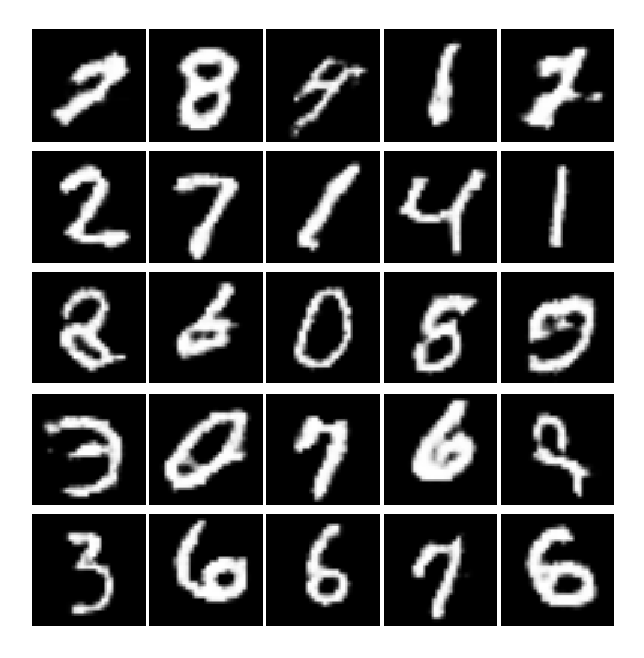
\includegraphics[width=.33\textwidth]{dcganmini005}
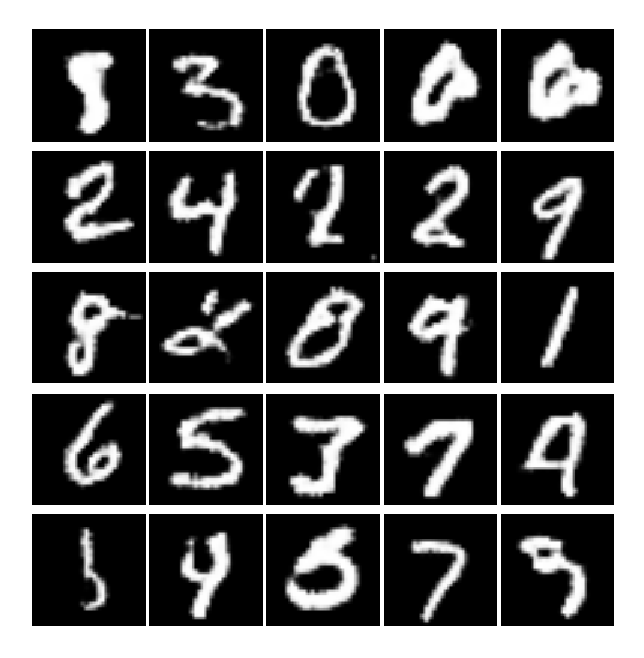
\includegraphics[width=.33\textwidth]{dcganmini010}
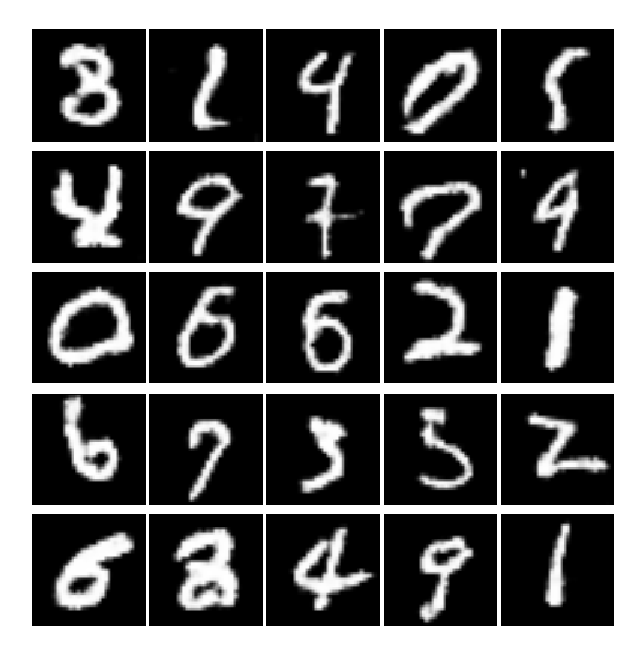
\includegraphics[width=.33\textwidth]{dcganmini020}
\end{center}
\caption{Uzorci nakon 0 (gore-lijevo), 25000 (gore-desno), 50000 (dolje-lijevo), 100000 (dolje-desno) iteracija (prvi model)}
\end{figure}

\begin{figure}[H]
\begin{center}
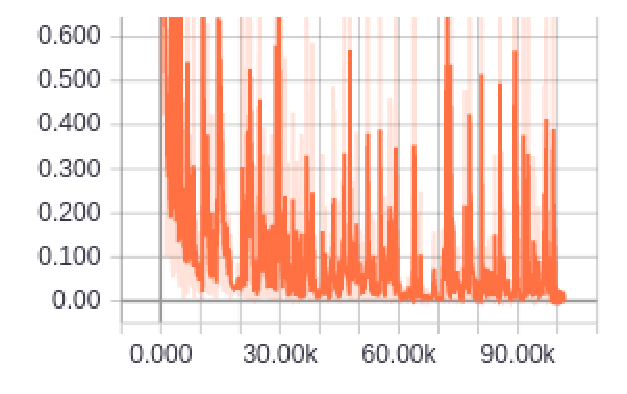
\includegraphics[width=.4\textwidth]{dcgandiscmini}
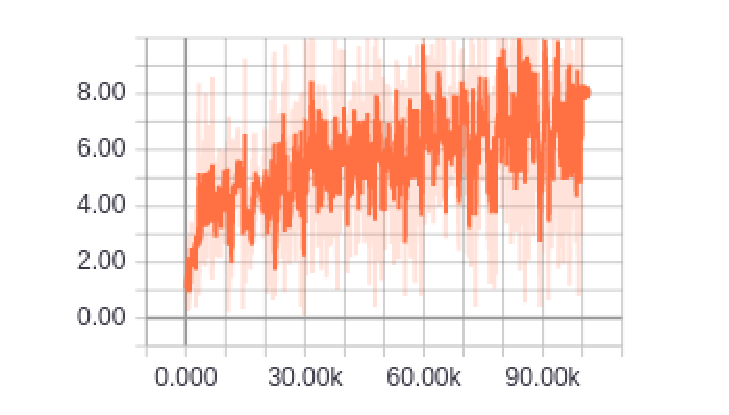
\includegraphics[width=.4\textwidth]{dcgangenmini}
\end{center}
\caption{Gubitak diskriminatora (lijevo) i generatora (desno) (prvi model)}
\end{figure}

Slika 4.7 prikazuje generirane slike nakon broja iteracija, slika 4.8 prikazuje gubitke generatora i diskriminatora kroz treniranje za četvrti model. Zaključak je da oba modela nemaju dovoljno velik kapacitet generatora, no da ipak donekle uspješno modeliraju distribuciju stvarnih podataka. Četvrti model ima generator malo većeg kapaciteta te se to odražava na gubitku generatora koji je u prosjeku manji nego kod prvog modela. Također, veza između gubitaka diskriminatora i generatora je inverzna, odnosno rastom jednog pada drugi, što je očekivano ponašanje.

\begin{figure}[H]
\begin{center}
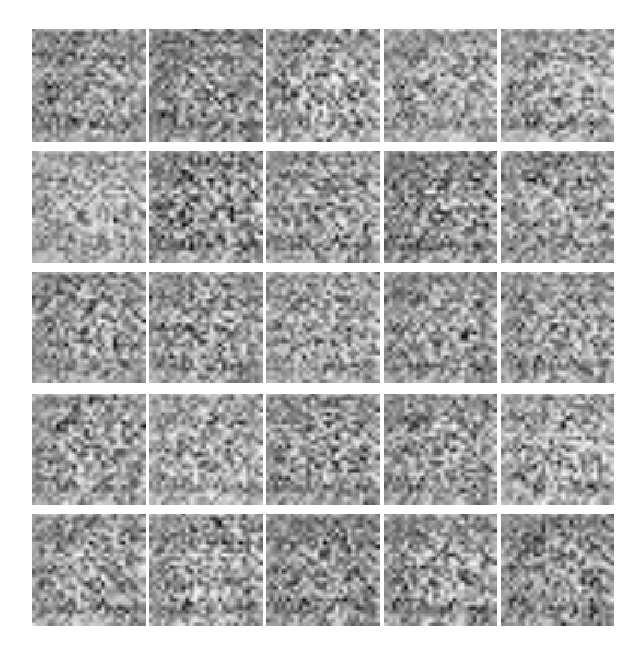
\includegraphics[width=.33\textwidth]{dcgan000}
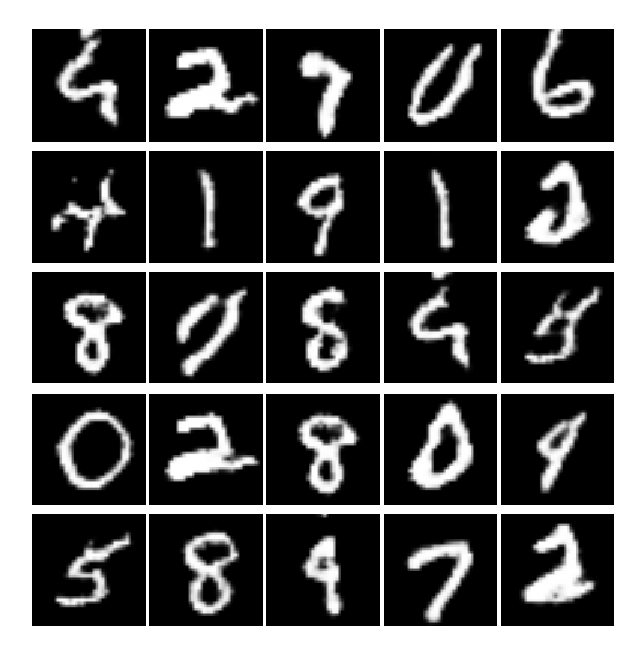
\includegraphics[width=.33\textwidth]{dcgan005}
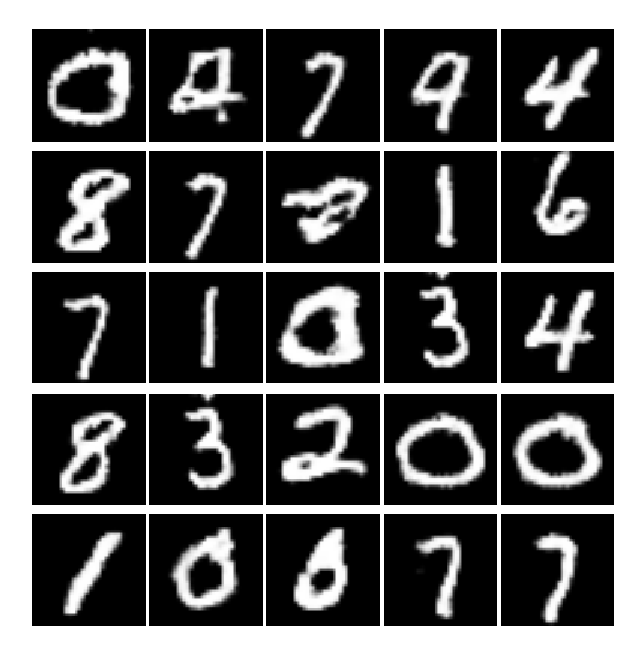
\includegraphics[width=.33\textwidth]{dcgan010}
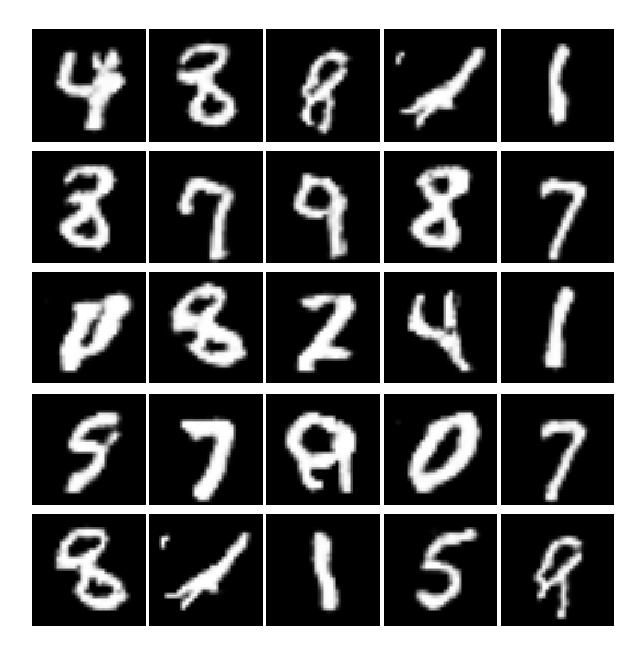
\includegraphics[width=.33\textwidth]{dcgan020}
\end{center}
\caption{Uzorci nakon 0 (gore-lijevo), 25000 (gore-desno), 50000 (dolje-lijevo), 100000 (dolje-desno) iteracija (četvrti model)}
\end{figure}

\begin{figure}[H]
\begin{center}
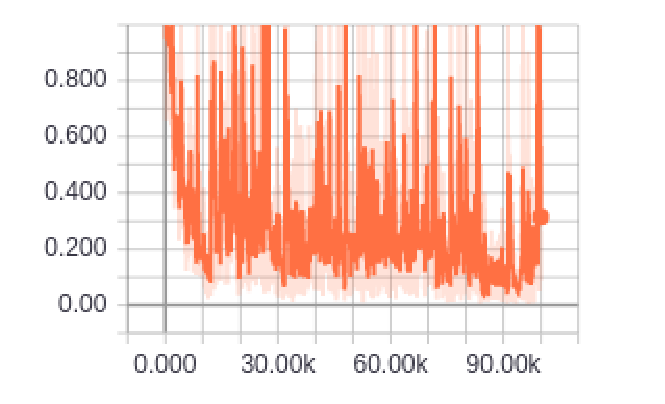
\includegraphics[width=.4\textwidth]{dcgandiscloss}
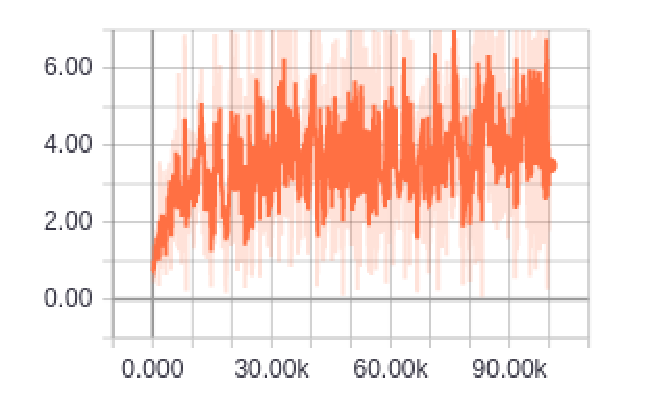
\includegraphics[width=.4\textwidth]{dcgangenloss}
\end{center}
\caption{Gubitak diskriminatora (lijevo) i generatora (desno) (četvrti model)}
\end{figure}

\subsection{Šetnja skrivenim prostorom}
Skriveni prostor je onaj prostor iz kojeg uzorkujemo šum. Proces učenja generatora je takav da mapira područja iz prostora šuma u prostor stvarnih podataka. Kvaliteta mapiranja ovisi o parametrima generatora. Duboki modeli općenito imaju velik kapacitet te su sposobni prenaučiti primjere preslikavanja. Stoga jedna od metoda validacije da naše učenje uči distribuciju pravih podataka i preslikavanje, a da ne pamti naslijepo primjere koje je vidio, zove se šetnja skrivenim prostorom. \par

Nasumično uzorkovanje vektora šuma kao što to radimo trenirajući generator ne daje nam dovoljnu validacijsku informaciju, pošto ti primjeri mogu biti zapamćeni. Stoga, odabire se skup kolinearnih točaka u latentnom prostoru te se nacrta preslikavanje koje se dobije kada ih se mapira u podatkovni prostor s generatorom. Očekuju se prijelazi između podataka, te doze neodređenosti između gdje se oblici mijenjaju. \par

Prvi način pronalaženja kolinearnih točaka je inicijalizacija jednog vektora šuma na [0 0 ... 0] te zatim stvaranje novih s pomakom, npr $0.05$, u oba smjera. Ilustracije radi drugi primjer bi izgledao [0.05 0.05 ... 0.05], a treći [-0.05 -0.05 ... -0.05]. Sve točke leže na istoj hiperravnini pošto su kolinearne, odnosno razlikuju se za faktor $k*pomak$. Slika 4.9 ilustrira ovakav način šetnje skrivenim prostorom. Iako se ne možemo sa sigurnošću reći koju točno regiju preslikavanja smo pogodili, da se naslutiti da smo zahvatili dio između broja $9$ i $0$, s potencijalno brojem $8$ između, te se vidi prijelaz u oblicima i neodređen dio u sredini.

\begin{figure}[H]
    \centering
    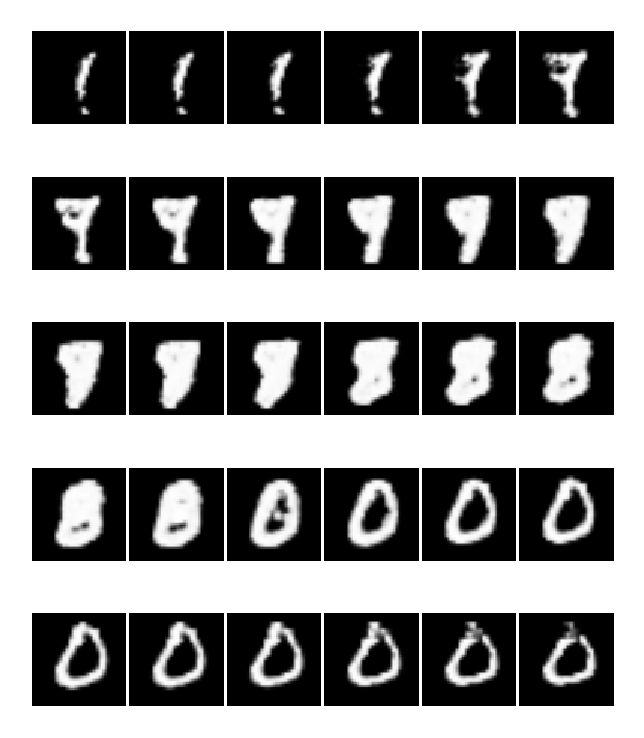
\includegraphics[scale=0.65]{Slike/latentwalk0}
    \caption{Primjer šetnje skrivenim prostorom}
\end{figure}

Drugi način pronalaženja kolinearnih točaka je inicijalizacija jednog vektora šuma tako da mu svih 100 vrijednosti bude u sitnom intervalu, primjerice [-0.05, 0.05]. Tada taj vektor uzastopno dodajemo i oduzimamo na vektor [0 0 ... 0], odnosno on postaje pomak. Nasumičnošću postižemo pogađanje različitih regija mapiranja, za  razliku od točnog određivanja svakog elementa vektora kojima šetamo. Svi ti vektori su kolinearni jer se razlikuju za faktor pomnožen s vektorom koji služi kao pomak. Slika 4.10 prikazuje rezultat ovakve šetnje. Pretpostavka je da je odabran dio preslikavanja broja $2$ te prijelaz u broj $9$, te između se nalazi regija neodređenosti.

\begin{figure}[H]
    \centering
    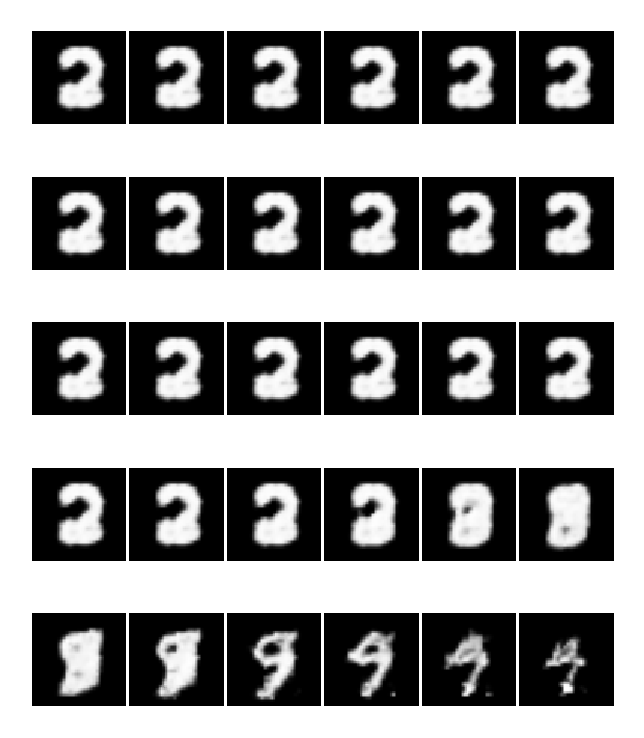
\includegraphics[scale=0.65]{Slike/latentwalk1}
    \caption{Primjer druge šetnje skrivenim prostorom}
\end{figure}

\subsection{Izvlačenje značajki}
Izvlačenje značajki je interesantno područje za provjeru kvalitete reprezentacija koje pronalaze nenadzirani modeli. Ideja je da se model trenira nenadzirano, da se zatim iz modela izvlače značajke koje je naučio nenadzirano i stave kao ulaz linearnom klasifikatoru, te se tako različiti nenadzirani modeli uspoređuju po kvaliteti naučenih reprezentacija. Linearni klasifikatori se koriste radi svog limitiranog kapaciteta, stoga rezultati će dati pravu sliku o značajkama, dok kad bi koristili modele visokog kapaciteta nikad ne bi znali da li su za dobar rezultat zaslužne značajke ili sam klasifikator. \par

Model koji je korišten u ovom eksperimentu je model dva, koji je identičan prvom modelu osim što ima jedan potpuno povezan sloj više. Stoga njegovo preslikavanje vektora šuma ne ide u skriveni sloj dimenzija 100x6272, već u prvi sloj 100x1024, a zatim u drugi sloj veličine 1024x6272, te se taj sloj preoblikuje u tenzor na isti način kao što je opisan prvi model. Svi ostali hiperparametri te inicijalizacije su identični. Nakon što je model naučen, zadnji sloj pred klasifikaciju diskriminatora je izvučen te se na temelju njega učilo linearne klasifikatore. Model je u potpunosti naučen nenadzirano. \par

Eksperimenti su obavljeni nad cijelim skupom za treniranje baze MNIST, nad 100 primjera po klasi (1000 primjera sveukupno), te na 10 primjera po klasi (100 primjera sveukupno). Svaki eksperiment je ponovljen 10 puta, da bi se dobila srednja vrijednost i varijanca samog postupka. Mjerena metrika je točnost klasifikacije. Mjereni su i rezultati linearnih klasifikatora nad pikselima slike, odnosno bez izvlačenja značajki. \par 

Osim usporedbe s linearnom klasifikacijom nad pikselima slike, usporedili smo model s još 2 modela. Za prvi model smo uzeli slučajno inicijalizirani diskriminator arhitekture koju koristimo i u DCGANu, te bez treniranja smo izvlačili njegovih 512 značajki i mjerili rezultate s linearnim klasifikatorima. Taj model bit će labeliran s RND. Za drugi model uzeli smo konvolucijsku neuronsku mrežu arhitekture diskriminatora te smo ju nadzirano trenirali s skupovima za učenje navedenima gore. Taj model nazvali smo Diskriminator.

\begin{table}[H]
\caption{Rezultati mjerenja za Linearni SVM}
\centering
\begin{tabular}{c c c c}
\hline\hline %inserts double horizontal lines
Klasifikator & Cijeli MNIST & 1000 primjera & 100 primjera \\ [0.5ex] % inserts table
%heading
\hline % inserts single horizontal line
LSVM (pikseli) & $91.75 \% \pm 0\%$ & $83.13 \% \pm 0\%$ & $72.2 \% \pm 0\%$ \\
LSVM (RND značajke) & $93.86 \% \pm 0.48\%$ & $83.55 \% \pm 1.15\%$ & $66.84 \% \pm 1.7\%$ \\
LSVM (DCGAN značajke) & $97.68 \% \pm 0.21\%$ & $92.99 \% \pm 0.45\%$ & $75.36 \% \pm 2\%$ \\
Diskriminator & $99.21 \% \pm 0.07\%$ & $91.14 \% \pm 2.6\%$ & $71.27 \% \pm 1.64\%$ \\ [1ex] % [1ex] adds vertical space
\hline %inserts single line
\end{tabular}
\end{table}

\begin{table}[H]
\caption{Rezultati mjerenja za Logističku regresiju}
\centering
\begin{tabular}{c c c c}
\hline\hline %inserts double horizontal lines
Klasifikator & Cijeli MNIST & 1000 primjera & 100 primjera \\ [0.5ex] % inserts table
%heading
\hline % inserts single horizontal line
LR (pikseli) & $91.98 \% \pm 0\%$ & $85.85 \% \pm 0\%$ & $73.15 \% \pm 0\%$ \\
LR (RND značajke) & $93.98 \% \pm 0.51\%$ & $85.11 \% \pm 1\%$ & $67.69 \% \pm 1.86\%$ \\
LR (DCGAN značajke) & $97.93 \% \pm 0.21\%$ & $93.74 \% \pm 0.44\%$ & $74.16 \% \pm 2.24\%$ \\
Diskriminator & $99.21 \% \pm 0.07\%$ & $91.14 \% \pm 2.6\%$ & $71.27 \% \pm 1.64\%$ \\ [1ex] % [1ex] adds vertical space
\hline %inserts single line
\end{tabular}
\end{table}

Tablica 4.1 prikazuje rezultate mjerenja gdje je za linearni klasifikator odabran linearni SVM, a tablica 4.2 prikazuje rezultate mjerenja gdje je linearan klasifikator logistička regresija. Korištene su zadane implementacije logističke regresije i linearnog klasifikatora iz scikit-learn python paketa. \par

Rezultati govore da ukoliko imamo velik broj označenih primjera, da su standardne nadzirane metode ispravan put u rješavanju klasifikacijskih problema. No, za manje označene skupove za učenje vidljiv je napredak u klasifikaciji naspram strogo nadziranog modela. Stoga, kombinacija nadziranog i nenadziranog učenja je idealna za situacije kada baza ima mnogo primjera za učenje, no kad ih je mali dio označen.

\subsection{Primjena na FM3 bazi slika}

Četvrti model je učen na FM3 bazi slika. Promjene u arhitekturi su nezamjetne, jedan dekonvolucijski sloj je promijenjen s dekonvolucijskog prozora veličine 7x7 na 8x8, te posljedično i onaj poslije njega s 14x14x1 na 16x16x3 da bi se dobila rezultirajuća slika 32x32x3. Prvi sloj diskriminatora ovog puta prima 3 ulazna kanala umjesto jednog (slike su u boji, a ne u sivoj skali poput MNISTa). Korišteno je 3222 primjera za učenje, veličina grupe 64, te se model trenirao 2000 epoha, približno 100000 iteracija. \par

\begin{figure}[H]
\begin{center}
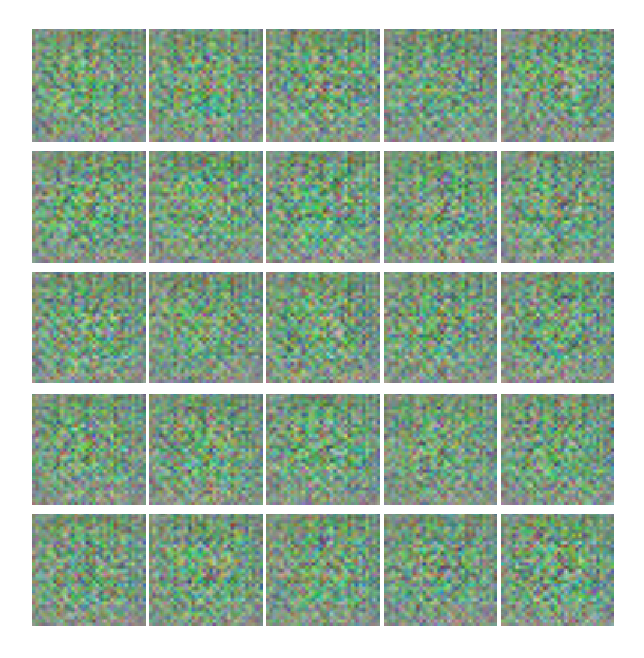
\includegraphics[width=.33\textwidth]{fm3000}
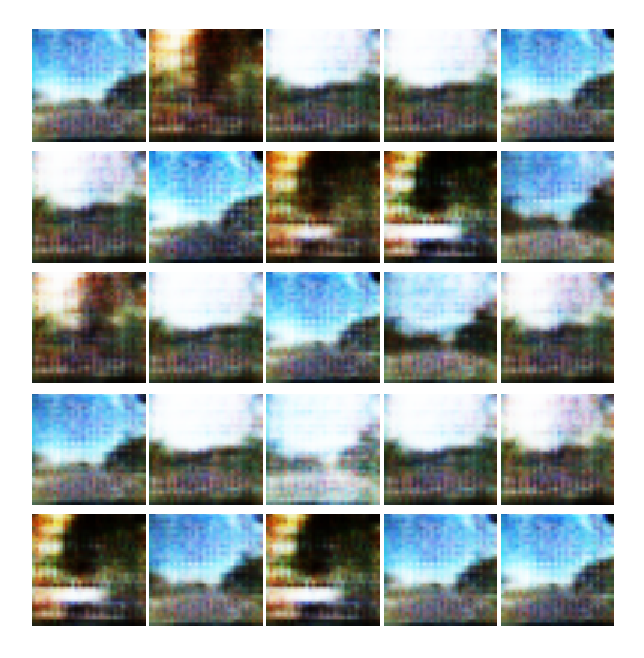
\includegraphics[width=.33\textwidth]{fm3005}
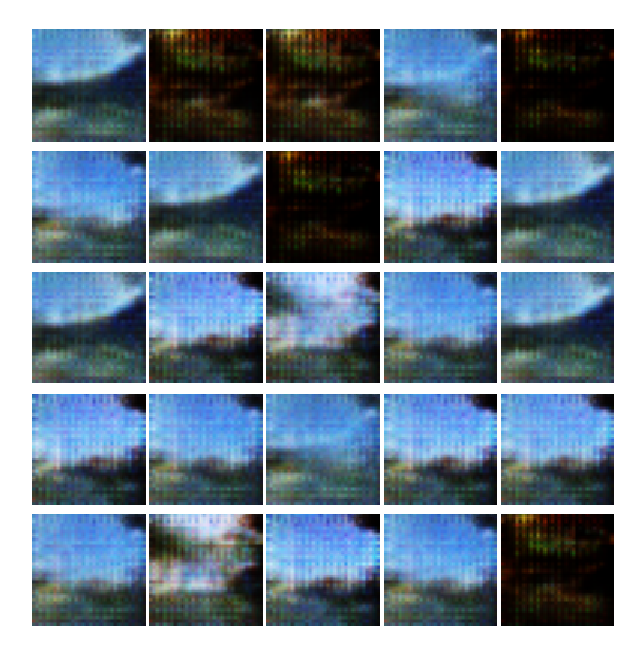
\includegraphics[width=.33\textwidth]{fm3010}
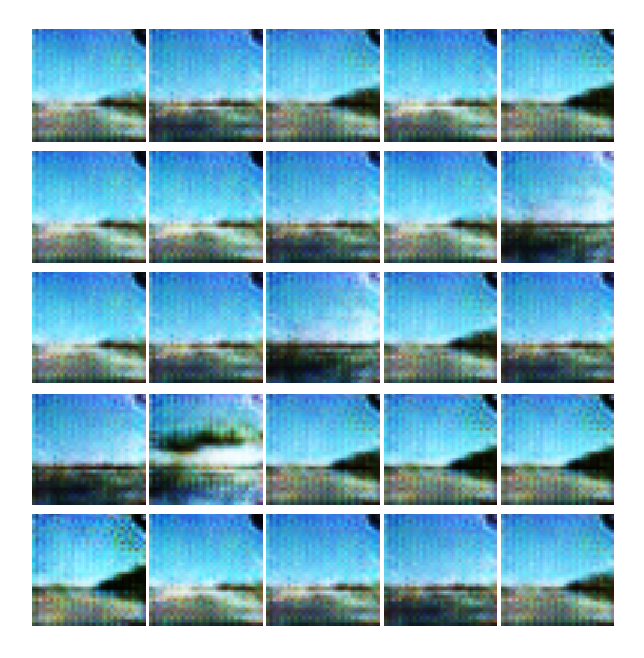
\includegraphics[width=.33\textwidth]{fm3020}
\end{center}
\caption{Uzorci nakon 0 (gore-lijevo), 25000 (gore-desno), 50000 (dolje-lijevo), 100000 (dolje-desno) iteracija}
\end{figure}

Na slici 4.11 su vidljivi artefakti, pojava pri preklapanju u dekonvoluciji \cite{artifacts}. Jedan od savjeta autora jest da se koriste dekonvolucijski prozori koji su višekratnici veličine koraka konvolucijskog prozora u generatoru, što je i istina za model u pitanju, no kako i oni kažu to nije garancija uklanjanja artefakata. Uklanjanje istih može biti smjernica za budući rad. \par

Model se koristio za izvlačenje značajki i usporedio pri klasifikaciji s običnim linearnim modelom. Klasifikacija je obavljena u \textit{jedan protiv ostalih} shemi u kojoj odabranu klasu uzimamo kao pozitivne primjere, a sve ostale za negativne te vršimo binarnu klasifikaciju po svih 8 klasa. Tablica 4.3 prikazuje metriku točnosti, gdje stupci odgovaraju klasi koja je uzeta kao pozitivan primjer. Za linearni model smo koristili linearni SVM u oba slučaja, jednom nad pikselima slike, a drugi put nad izvučenim značajkama.

\begin{table}[H]
\caption{Rezultati mjerenja točnosti}
\small
\centering
\begin{tabular}{c c c c c c c c c}
\hline\hline %inserts double horizontal lines
  & 0 & 1  & 2 & 3 & 4 & 5 & 6 & 7 \\ [0.5ex] 
\hline % inserts single horizontal line
pikseli & $93.51\%$ & $94.94\%$ & $99.32\%$ & $99.44\%$ & $95.71\%$ & $97.80\%$ & $98.60\%$ & $98.70\%$ \\
značajke & $95.16\%$ & $94.63\%$ & $99.41\%$ & $99.81\%$ & $96.40\%$ & $98.85\%$ & $98.85\%$ & $98.66\%$ \\ [1ex] % [1ex] adds vertical space
\hline %inserts single line
\end{tabular}
\end{table}

Rad sa značajkama je marginalno bolji, u nekim slučajevima možda i gori. Pretpostavljamo da je to do metrike točnosti, pošto je u ovom slučaju nesrazmjer u broju pozitivnih i negativnih primjera, stoga su istražene metrike preciznost i odziva u Tablicama 4.4 i 4.5. \par

\begin{table}[H]
\caption{Rezultati mjerenja preciznosti}
\small
\centering
\begin{tabular}{c c c c c c c c c}
\hline\hline %inserts double horizontal lines
  & 0 & 1  & 2 & 3 & 4 & 5 & 6 & 7 \\ [0.5ex] 
\hline % inserts single horizontal line
pikseli & $91.05\%$ & $63.52\%$ & $95.56\%$ & $71.43\%$ & $72.50\%$ & $33.33\%$ & $65.96\%$ & $66.67\%$ \\
značajke & $95.74\%$ & $69.41\%$ & $95.90\%$ & $92.31\%$ & $76.92\%$ & $78.05\%$ & $72.00\%$ & $65.38\%$ \\ [1ex] % [1ex] adds vertical space
\hline %inserts single line
\end{tabular}
\end{table}

\begin{table}[H]
\caption{Rezultati mjerenja odziva}
\small
\centering
\begin{tabular}{c c c c c c c c c}
\hline\hline %inserts double horizontal lines
  & 0 & 1  & 2 & 3 & 4 & 5 & 6 & 7 \\ [0.5ex] 
\hline % inserts single horizontal line
pikseli & $95.78\%$ & $68.77\%$ & $97.42\%$ & $89.74\%$ & $70.80\%$ & $24.56\%$ & $55.17\%$ & $55.93\%$ \\
značajke & $97.11\%$ & $65.80\%$ & $98.06\%$ & $92.31\%$ & $75.60\%$ & $56.14\%$ & $62.07\%$ & $55.93\%$ \\ [1ex] % [1ex] adds vertical space
\hline %inserts single line
\end{tabular}
\end{table}

\section{Klasifikatorska generativna suparnička mreža}
Klasifikatorska generativna suparnička mreža koristi arhitekturu identičnu drugom modelu, osim što diskriminator ima 2 izlaza, za nadzirano i nenadzirano učenje. Cijeli model je strogo nadziran, odnosno bez modifikacija ne može raditi s neoznačenim primjerima. Za nadzirano učenje izlaz ima 10 \textit{softmax} (praktički, višeklasna logistička regresija) neurona, za nenadzirano ima standardni sigmoidalni neuron. Slika 4.12 prikazuje generirane primjere. Naočigled, primjeri su puno više nalik stvarnima, što i ima smisla pošto generatorski prostor dijelimo i po oznakama, stoga je zadatak generatora uvelike olakšan. \par

\begin{figure}[H]
\begin{center}
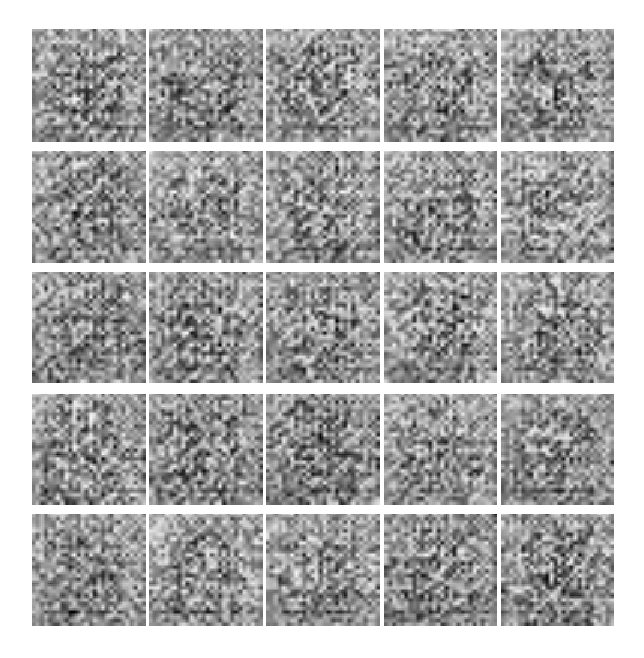
\includegraphics[width=.33\textwidth]{ACGAN000}
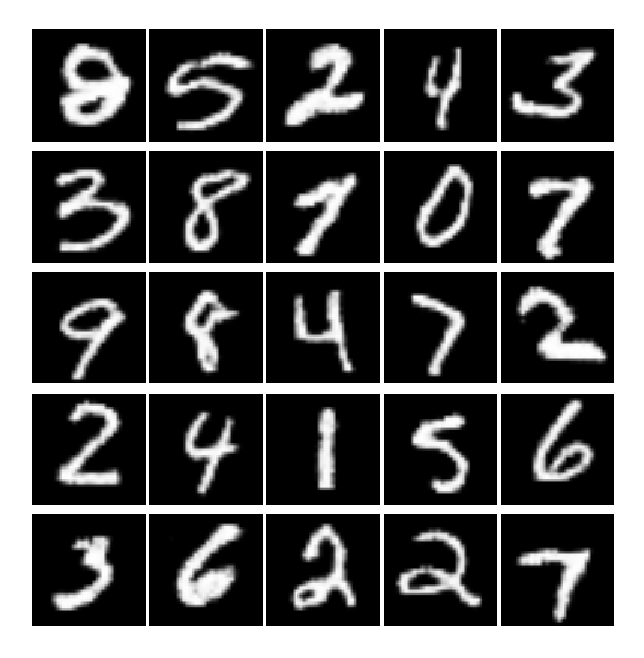
\includegraphics[width=.33\textwidth]{ACGAN005}
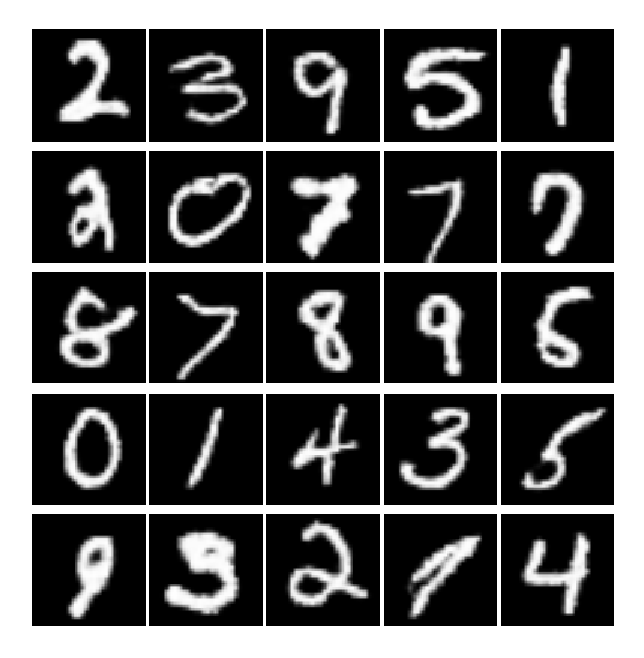
\includegraphics[width=.33\textwidth]{ACGAN010}
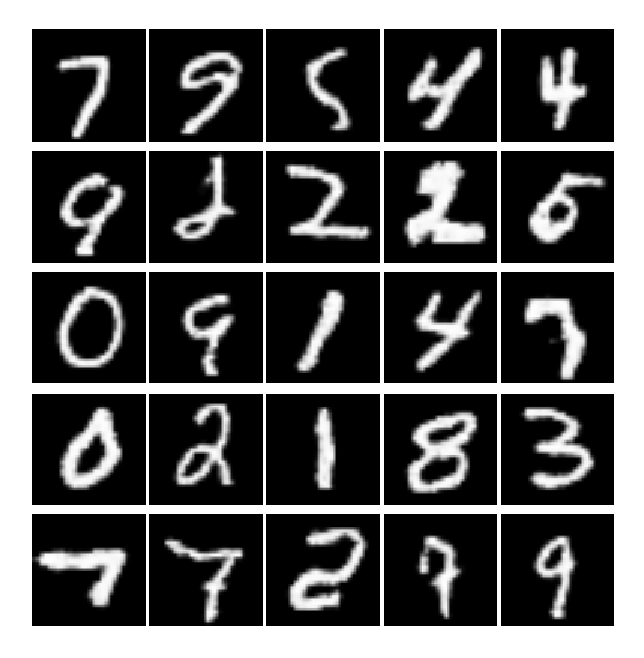
\includegraphics[width=.33\textwidth]{ACGAN020}
\end{center}
\caption{Uzorci nakon 0 (gore-lijevo), 25000 (gore-desno), 50000 (dolje-lijevo), 100000 (dolje-desno) iteracija}
\end{figure}

Provedeni su i klasifikacijski eksperimenti te su uspoređeni s zasebnom mrežom diskriminatora koja je učena označenim primjerima. Kako klasifikatorska generativna suparnička mreža ima nadzirani i nenadzirani gubitak, pretpostavka je da će pri optimizaciji nenadzirani gubitak štetiti nadziranom i obratno, stoga je proveden eksperiment gdje se težine diskriminatora uče otežano, odnosno faktor $0.9$ se nalazi uz nadzirani gubitak, a faktor $0.1$, uz nenadzirani, što bi optimizacijski postupak nagnalo da težine gura ka smanjivanju klasifikacijske greške. Rezultati su prikazani u tablici 4.6. Klasifikatorska generativna suparnička mreža se referira kao AC-GAN, model s otežanim klasifikacijskim gubitkom je Weighted AC-GAN, a Diskriminator označava zasebnu mrežu arhitekture diskriminatora. \par

\begin{table}[H]
\caption{Rezultati mjerenja za klasifikatore}
\centering
\begin{tabular}{c c c c}
\hline\hline %inserts double horizontal lines
Klasifikator & Cijeli MNIST & 1000 primjera & 100 primjera \\ [0.5ex] % inserts table
%heading
\hline % inserts single horizontal line
AC-GAN & $98.56\%$ & $75.48\%$ & $16.4\%$ \\
Weighted AC-GAN & $99.21\%$ & $88.65\%$ & $22.13\%$ \\
Diskriminator & $99.2\%$ & $91.89\%$ & $75.4\%$ \\ [1ex] % [1ex] adds vertical space
\hline %inserts single line
\end{tabular}
\end{table}

Pretpostavke su se ispostavile ispravnima, nenadzirani gubitak šteti klasifikaciji modela. Podrobniji eksperimenti nisu potrebni pošto se model nije pokazao superiornijim običnom klasifikatoru stoga je jedina prednost ovog modela bolji generirani uzorci te mogućnost uvjetovanja uzorkovanja, odnosno može se od modela zatražiti primjere odabrane klase. Slika 4.13 prikazuje generirane slike Weighted AC-GANa, očekivano su slabije kvalitete pošto je manji faktor uz nenadzirani gubitak.

\begin{figure}[H]
\begin{center}
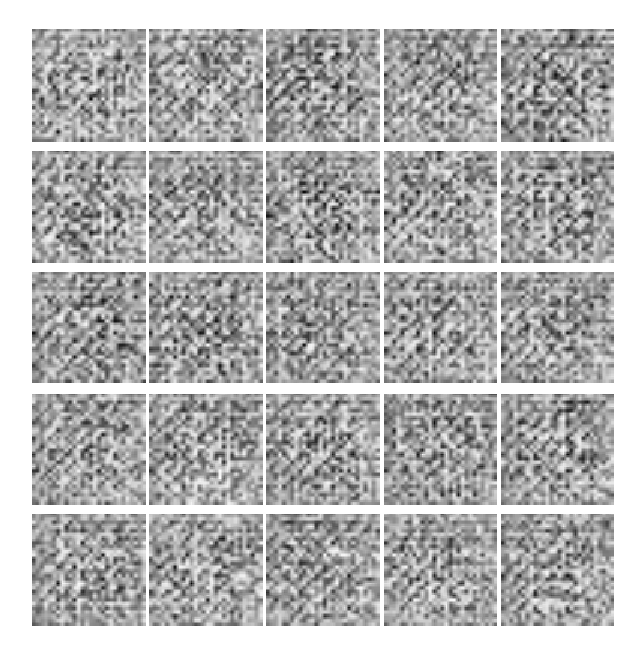
\includegraphics[width=.33\textwidth]{wacgan000}
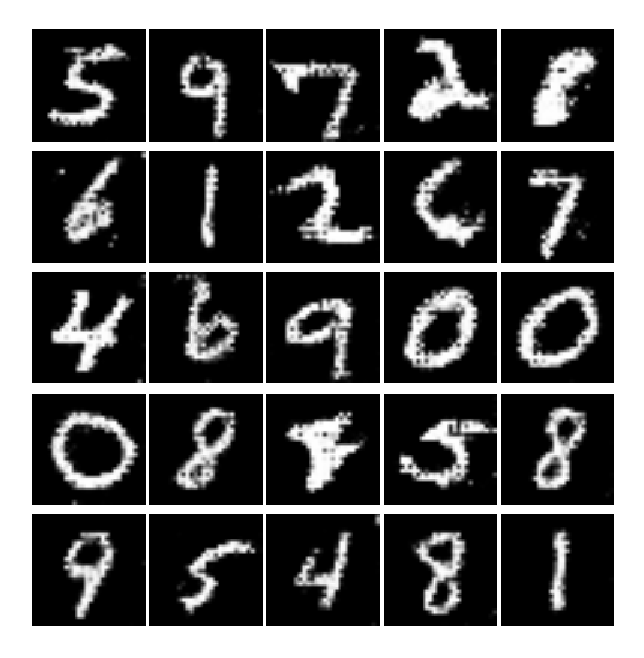
\includegraphics[width=.33\textwidth]{wacgan005}
\includegraphics[width=.33\textwidth]{wacgan010}
\includegraphics[width=.33\textwidth]{wacgan020}
\end{center}
\caption{Uzorci nakon 0 (gore-lijevo), 25000 (gore-desno), 50000 (dolje-lijevo), 100000 (dolje-desno) iteracija}
\end{figure}




\chapter{Zaključak}
Ubrzani razvoj na području dubokog učenja luči skoro pa svakodnevne napretke i sve širu primjenu. U ovom radu opisane su neuronske mreže kroz povijest te je objašnjena pojava dubokih modela neuronskih mreža, kao i svih najvažnijih pojmova vezanih za suvremene duboke neuronske mreže. \par

U sklopu rada implementirano je više inačica generativnih suparničkih mreža u radnom okviru \textit{Tensorflow} s podrškom za CUDA procesiranje koji je otvoren za korištenje svima te se kontinuirano nadograđuje. \par

Generativne suparničke mreže su se pokazale kao jedan od najpopularnijih modernih modela čije nove inačice izlaze gotovo na tjednoj bazi. Ovaj rad pruža uvid u nekoliko najbitnijih takvih inačica, njihove arhitekture, hiperparametre i rezultate. Prikazana je i njegova primjena kao nenadziranog modela u nadziranoj klasifikaciji, gdje potencijalno pronalazi primjenu u polunadziranom učenju, kada na raspolaganju imamo mnogo primjera, ali malo označenih. \par

Odabir arhitektura generatora i diskriminatora se pokazao ključnim u uspješnosti učenja modela, stoga u budućnosti očekujemo stabilnije modifikacije modela koji su manje osjetljivi na arhitekturu te napredak po pitanju kriterija konvergencije modela. \par

\bibliography{literatura}
\bibliographystyle{fer}

\begin{sazetak}
U radu su opisane neuronske mreže, metode učenja neuronskih mreža te je dan uvid u najpoznatije moderne arhitekture, s naglaskom na generativnim suparničkim mrežama. Implementirano je više inačica spomenutog modela u \textit{Tensorflow} radnom okviru te su modeli testirani na 2 skupa podataka, MNIST i FM3. Tablicama i slikama su prikazani klasifikacijski i generativni rezultati. Model se pokazao korisnim u polunadziranom okruženju, kada služi za izvlačenje značajki u nenadziranom okruženju, te prosljeđivanju istih nadziranom modelu. 

\kljucnerijeci{Neuronske mreže, generativne suparničke mreže, polunadzirana klasifikacija}
\end{sazetak}

% TODO: Navedite naslov na engleskom jeziku.
\engtitle{Semisupervised classification of handwritten characters using generative adversarial models}
\begin{abstract}
This paper describes neural networks, methods on training neural networks and it provides an insight to the most famous modern architectures, with emphasis on generative adversarial networks. A few versions of the aforementioned model have been implemented in \textit{Tensorflow} framework, with models being trained on 2 datasets, MNIST and FM3. Tables and figures provide insight to classification and generative results. Model has proven useful in a semisupervised environment, when a large dataset is available but only a fraction of it has been labeled.

\keywords{Neural networks, generative adversarial networks, semisupervised classification}
\end{abstract}

\end{document}
